\documentclass[11pt,a4paper]{article}

\usepackage[margin=2.5cm]{geometry}
\usepackage{amsmath,amssymb,amsthm}
\usepackage{booktabs}
\usepackage{array}
\usepackage{hyperref}
\usepackage{microtype}
\usepackage{xcolor}
\usepackage{multirow}
\usepackage{enumitem}
\usepackage{tikz}
\usepackage[most]{tcolorbox}
\usepackage{caption}
\usepackage{graphicx}
\usepackage{subcaption}
\graphicspath{{../individual_graphs/}}

\usetikzlibrary{positioning, calc, decorations.pathmorphing}

% ---------- theorem environments ----------
\theoremstyle{plain}
\newtheorem{theorem}{Theorem}[section]
\newtheorem{proposition}[theorem]{Proposition}
\newtheorem{corollary}[theorem]{Corollary}
\newtheorem{lemma}[theorem]{Lemma}
\newtheorem{conjecture}[theorem]{Conjecture}

\theoremstyle{definition}
\newtheorem{definition}[theorem]{Definition}
\newtheorem{example}[theorem]{Example}
\newtheorem{construction}[theorem]{Construction}
\newtheorem{observation}[theorem]{Observation}

\theoremstyle{remark}
\newtheorem{remark}[theorem]{Remark}

% ---------- convenience macros ----------
\newcommand{\Z}{\mathbb{Z}}
\newcommand{\R}{\mathbb{R}}
\newcommand{\C}{\mathbb{C}}
\newcommand{\Q}{\mathbb{Q}}
\newcommand{\F}{\mathbb{F}}
\newcommand{\N}{\mathbb{N}}
\newcommand{\Aut}{\operatorname{Aut}}
\newcommand{\PSL}{\operatorname{PSL}}
\newcommand{\PGL}{\operatorname{PGL}}
\newcommand{\SU}{\operatorname{SU}}
\newcommand{\PSU}{\operatorname{PSU}}
\newcommand{\Sab}{\operatorname{Sab}}
\newcommand{\Spec}{\operatorname{Spec}}
\newcommand{\tr}{\operatorname{tr}}
\newcommand{\GH}{\mathrm{GH}(2,2)}
\newcommand{\Gtwo}{G_2(2)}
\newcommand{\CR}{\mathrm{CR}}
\newcommand{\GP}{\mathrm{GP}}
\newcommand{\lmin}{\lambda_{\min}}

\title{\textbf{Spectral Programme:\\
  Eigenvalues of Arc-Transitive Graphs\\
  from Groups of Lie Type}}
\author{Robin Langer}
\date{August 2026}

\begin{document}
\maketitle

\begin{abstract}
We present a unified spectral survey of 30+ graphs arising from the
programme of constructing arc-transitive graphs as Sabidussi
coset graphs of groups of Lie type. The survey spans five families:
the Foster census (13 small cubic arc-transitive graphs), the
$\PSL(2,q)$ tower (7 cubic graphs from $\SU(2)$ over finite fields),
the exceptional Lie group $G_2(2)$ (3 graphs of varying regularity),
voltage covers via cubic residues (6 bipartite lifts),
and hypercubes $Q_n$ (as a contrast from abelian groups).
Every graph from a simple Lie-type group in the census is Ramanujan
for its degree, a phenomenon we trace to the Weil conjectures.
Cross-family comparison reveals universal structural patterns:
eigenvalues in small algebraic number fields,
Fiedler values decaying as $O(1/q)$, eigenvalue multiplicities
governed by the representation theory of the acting group,
and a spectral--geometric dictionary linking algebraic and
combinatorial properties.
\end{abstract}

\tableofcontents

\bigskip

% ======================================================================
%
%  PART I: SYNTHESIS
%
% ======================================================================

\part*{Part I: Synthesis}
\addcontentsline{toc}{part}{Part I: Synthesis}

% ==========================================================================
\section{Introduction}
% ==========================================================================

The Sabidussi construction $\Sab(G, H, HaH)$ builds a graph from a group
$G$, a subgroup $H$, and a double coset $HaH$: the vertices are cosets
$G/H$ and two cosets $Hx$, $Hy$ are adjacent iff $xy^{-1} \in HaH$. When
$|HaH|/|H| = 3$, the result is a cubic (3-regular) graph; when $G$ acts
arc-transitively, the graph is arc-transitive.

This paper synthesises spectral data from a computational census of such
graphs, focusing on four families of Lie-type origin plus hypercubes as a
contrasting abelian family.
Each family is treated in its own Part; here we extract the
cross-cutting themes.

\begin{tcolorbox}[breakable, colback=yellow!10, colframe=yellow!10,
  boxrule=0pt, sharp corners]
\textbf{The programme at a glance.}
The five families are:
\begin{enumerate}[noitemsep]
\item \textbf{Foster census} (Part~II) --- the 13 smallest cubic arc-transitive
  graphs ($|V| \le 30$), all computable without group theory.
\item \textbf{$\PSL(2,q)$ family} (Part~III) --- cubic Sabidussi graphs from the
  $A_1$ Lie type, with stabilisers $H \in \{C_3, S_3, S_4\}$.
\item \textbf{$G_2(2)$ family} (Part~IV) --- three graphs (cubic, 6-regular,
  7-regular) from the smallest exceptional Lie group.
\item \textbf{Voltage graphs} (Part~V) --- cyclic covers $\Z_p \to K_2$ with cubic
  residue voltages, connecting number theory to graph spectra.
\item \textbf{Hypercubes} (Part~VI) --- $Q_n = K_2^{\square n}$, the abelian
  Cayley graphs, as a contrast and complement.
\end{enumerate}
\end{tcolorbox}


\begin{figure}[htbp]
\centering
\begin{subfigure}[b]{0.3\textwidth}
  \centering
  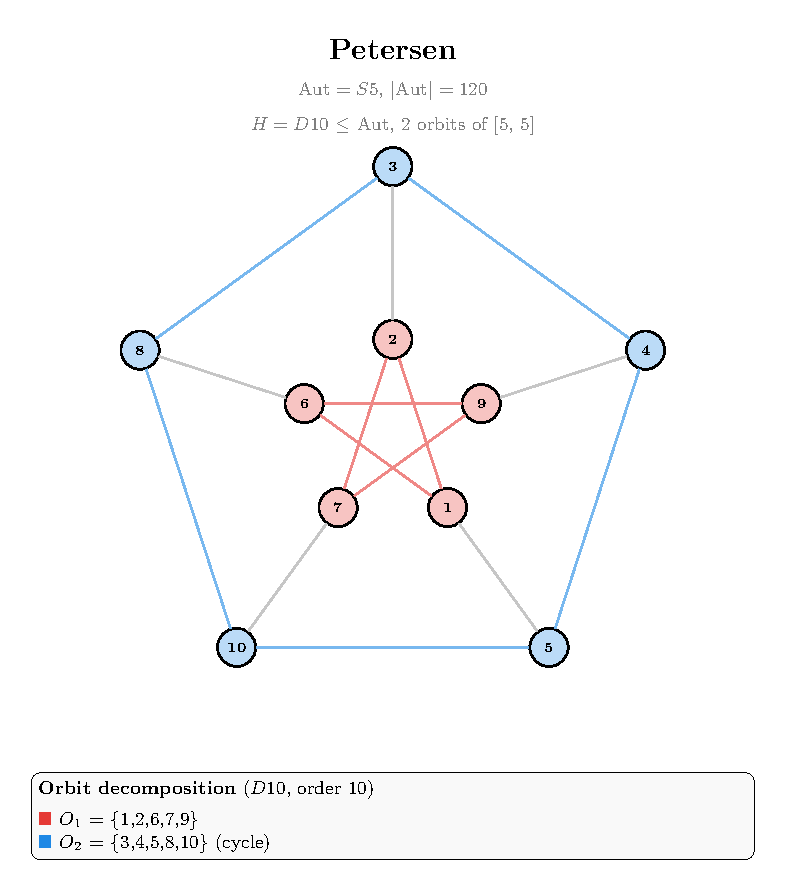
\includegraphics[width=\textwidth]{auto-petersen.pdf}
  \caption{Petersen ($\PSL(2,5)/S_3$)}
\end{subfigure}\hfill
\begin{subfigure}[b]{0.3\textwidth}
  \centering
  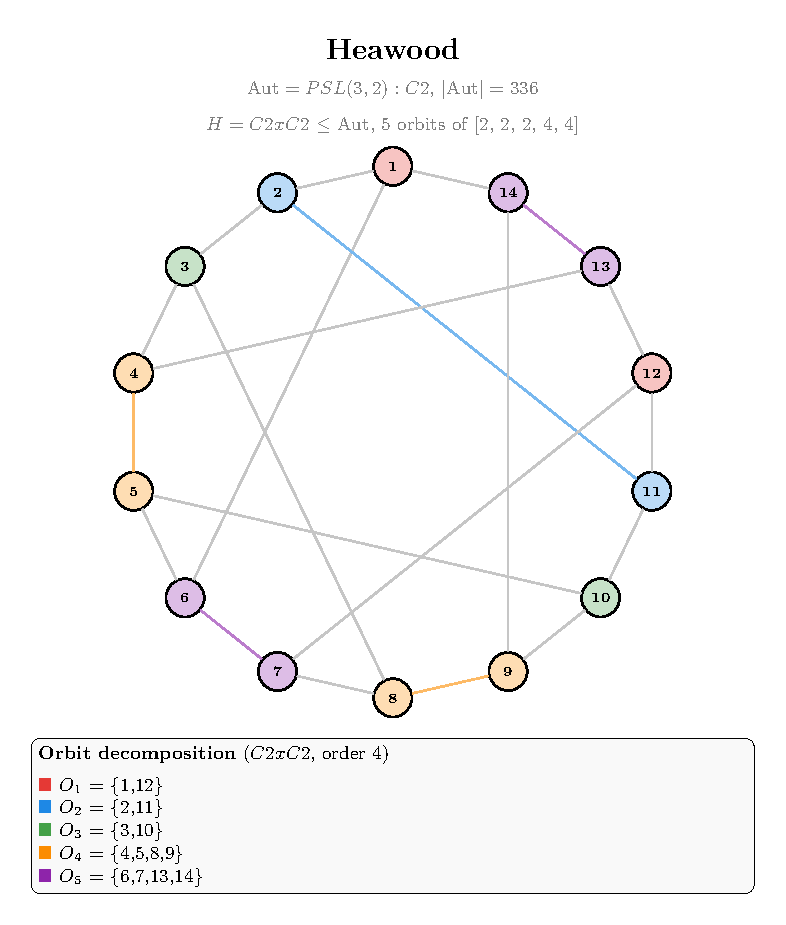
\includegraphics[width=\textwidth]{auto-heawood.pdf}
  \caption{Heawood ($\PGL(2,7)/S_4$)}
\end{subfigure}\hfill
\begin{subfigure}[b]{0.3\textwidth}
  \centering
  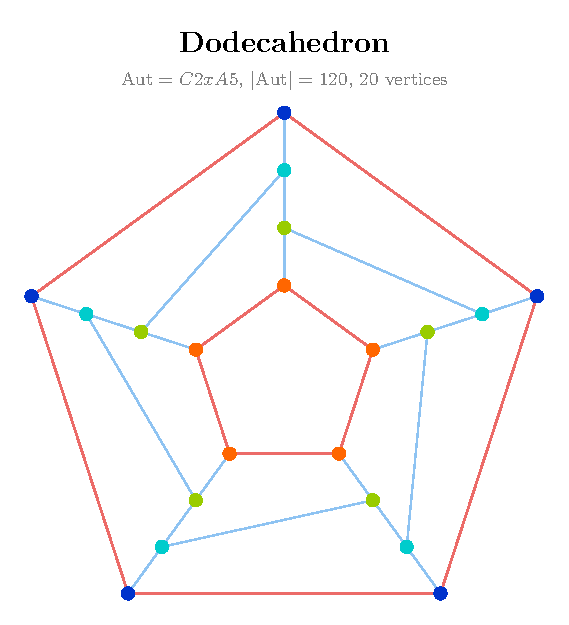
\includegraphics[width=\textwidth]{auto-dodecahedron.pdf}
  \caption{Dodecahedron ($A_5$)}
\end{subfigure}

\medskip
\begin{subfigure}[b]{0.3\textwidth}
  \centering
  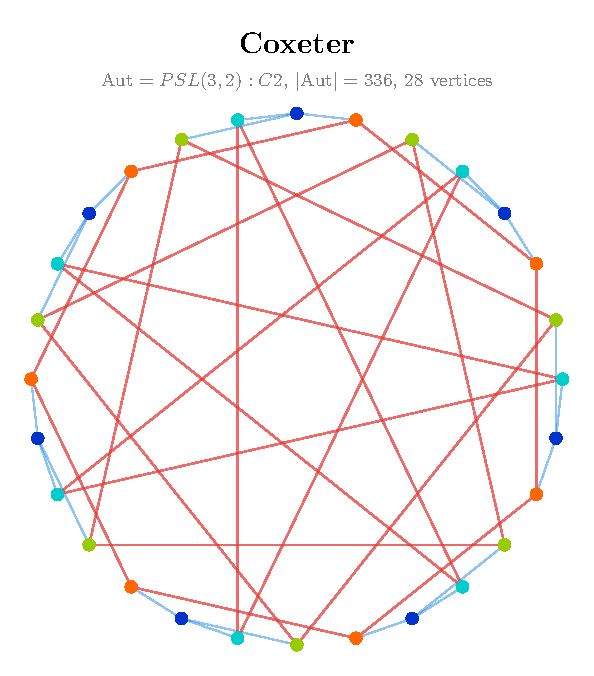
\includegraphics[width=\textwidth]{auto-coxeter.pdf}
  \caption{Coxeter (28 vertices)}
\end{subfigure}\hfill
\begin{subfigure}[b]{0.3\textwidth}
  \centering
  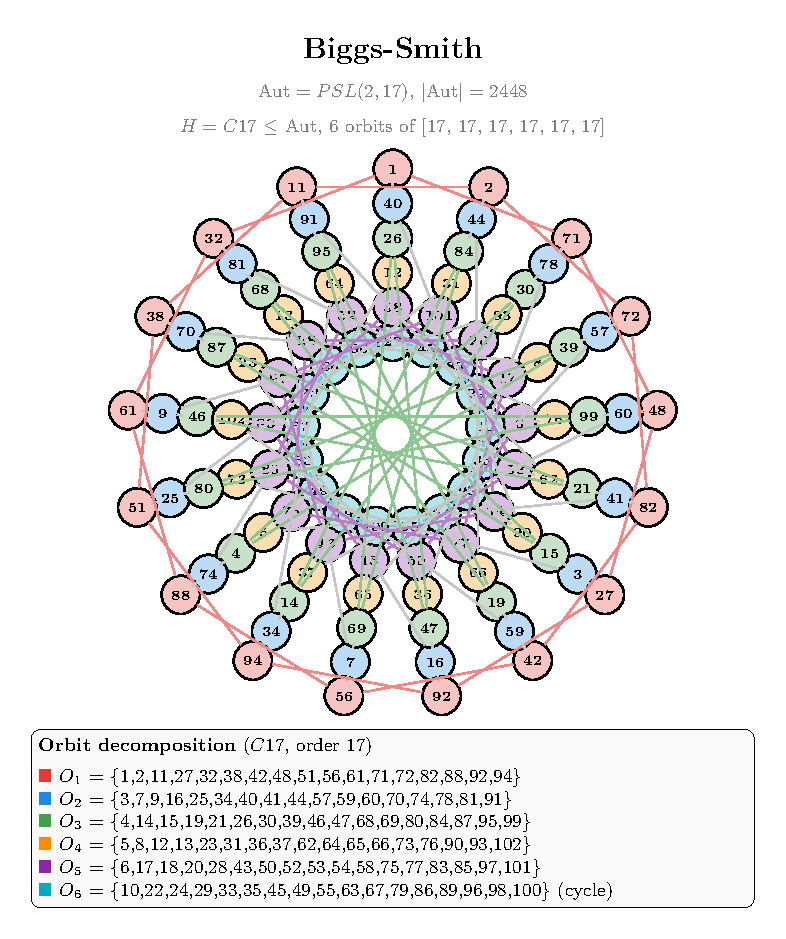
\includegraphics[width=\textwidth]{auto-biggssmith.pdf}
  \caption{Biggs-Smith ($\PSL(2,17)/S_4$)}
\end{subfigure}\hfill
\begin{subfigure}[b]{0.3\textwidth}
  \centering
  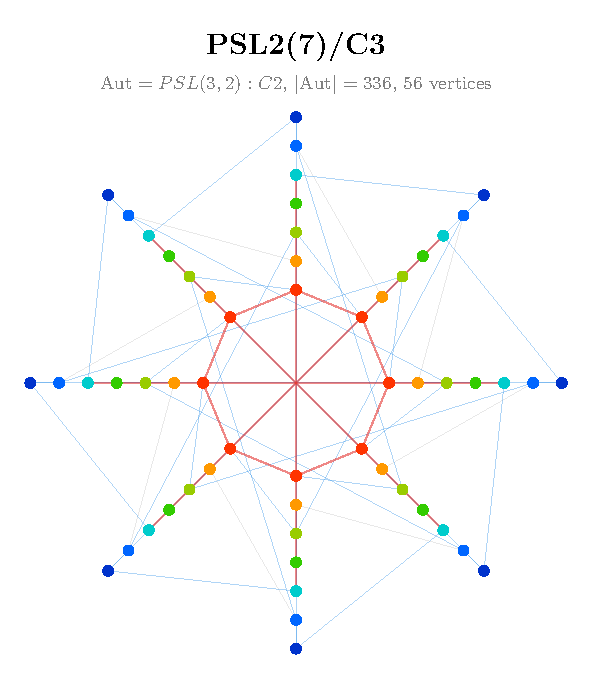
\includegraphics[width=\textwidth]{auto-psl2_7_c3.pdf}
  \caption{Klein ($\PSL(2,7)/C_3$)}
\end{subfigure}
\caption{Six graphs from the spectral programme, drawn with symmetry-aware
  layout. Each drawing uses the automorphism group to place vertices on
  concentric rings with rotational symmetry.}
\label{fig:showcase}
\end{figure}


% ==========================================================================
\section{The universal Ramanujan phenomenon}
% ==========================================================================

\begin{tcolorbox}[colback=green!8, colframe=green!8,
  boxrule=0pt, sharp corners]
\begin{definition}
A connected $d$-regular graph is \emph{Ramanujan} if every nontrivial
eigenvalue $\lambda$ (i.e., $|\lambda| < d$) satisfies
$|\lambda| \le 2\sqrt{d-1}$.
\end{definition}
\end{tcolorbox}

\begin{tcolorbox}[breakable, colback=black!5, colframe=black!5,
  boxrule=0pt, sharp corners]
\begin{theorem}[Computational]
\label{thm:all-ramanujan}
Every graph from a simple Lie-type group in the census is Ramanujan for its degree:
\begin{itemize}[noitemsep]
\item All 13 Foster census graphs (cubic, bound $2\sqrt{2} \approx 2.828$).
\item All 7 $\PSL(2,q)$ Sabidussi graphs (cubic).
\item The Tutte 12-cage (cubic, $\lambda_2 = \sqrt{6} \approx 2.449 < 2\sqrt{2} \approx 2.828$).
\item The $\GH$ collinearity graph (6-regular, $\lambda_2 = 3$
  vs.\ bound $2\sqrt{5} \approx 4.472$).
\item The Meinhold-72 graph (7-regular, $\lambda_2 = \sqrt{13} \approx 3.606$
  vs.\ bound $2\sqrt{6} \approx 4.899$).
\item All 6 cubic residue voltage lifts $\CR(p)$
  ($p = 7, 13, 19, 31, 37, 43$).
\end{itemize}
All three $G_2(2)$ graphs are Ramanujan. The hypercubes $Q_n$ are Ramanujan
for $n \le 6$ but fail at $n = 7$ (see Part~VI).
\end{theorem}
\end{tcolorbox}

\begin{tcolorbox}[breakable, colback=yellow!10, colframe=yellow!10,
  boxrule=0pt, sharp corners]
\textbf{Why universality?}
This is not a coincidence. For the $\PSL(2,q)$ family, the
Ramanujan property follows from Deligne's proof of the Weil conjectures:
the nontrivial eigenvalues of a Hecke operator on $\mathrm{GL}(2)$ over
a function field are bounded by $2\sqrt{q}$, and the graph eigenvalues
are evaluations of these operators at specific representations.
The Lubotzky--Phillips--Sarnak construction~\cite{LPS} made this
connection explicit for Cayley graphs of $\PSL(2,q)$.

For the voltage lifts, the eigenvalues are Gauss-type character sums
$f_j = \sum_{v \in V} \omega^{jv}$ where $V$ is the set of cubic residues
and $\omega = e^{2\pi i/p}$. The Weil bound gives
$|f_j| \le 2\sqrt{p}$ for nontrivial characters, which after normalisation
yields $\lambda_2 \le 2\sqrt{2}$.
\end{tcolorbox}

\begin{tcolorbox}[colback=black!5, colframe=black!5,
  boxrule=0pt, sharp corners]
\begin{observation}
The $G_2(2)$ graphs are Ramanujan despite coming from an exceptional Lie
group rather than a classical one. This suggests the Ramanujan property
may extend beyond the $A_1$ setting to all Chevalley groups, at least for
small field sizes.
\end{observation}
\end{tcolorbox}


% ==========================================================================
\section{Master spectral table}
\label{sec:master-table}
% ==========================================================================

Table~\ref{tab:master} collects the key spectral invariants across all
families. Graphs are grouped by family and sorted by vertex count within
each family. Detailed spectra appear in the individual Parts.

\begin{tcolorbox}[breakable, colback=black!5, colframe=black!5,
  boxrule=0pt, sharp corners]
\centering
\captionof{table}{Spectral invariants of all graphs in the census.
  $d$ = degree, $g$ = girth, $\lambda_2$ = second-largest adjacency eigenvalue,
  $\mu_1$ = Fiedler (algebraic connectivity), \#$\lambda$ = number of
  distinct eigenvalues. All Lie-type graphs are Ramanujan.}
\label{tab:master}
\smallskip
\renewcommand{\arraystretch}{1.05}
\small
\begin{tabular}{@{}l r r r r r r l@{}}
\toprule
Graph & $|V|$ & $d$ & $g$ & $\lambda_2$ & $\mu_1$ & \#$\lambda$ & Source \\
\midrule
\multicolumn{8}{@{}l}{\textit{Foster census (Part~II)}} \\
$K_4$         &   4 & 3 & 3 & $-1.000$ & $4.000$ &  2 & \\
$K_{3,3}$     &   6 & 3 & 4 & $0.000$  & $3.000$ &  3 & \\
Cube $Q_3$    &   8 & 3 & 4 & $1.000$  & $2.000$ &  4 & $\Z_2^3$ \\
Petersen      &  10 & 3 & 5 & $1.000$  & $2.000$ &  3 & $\PSL(2,5)/S_3$ \\
Heawood       &  14 & 3 & 6 & $\sqrt{2}$  & $1.586$ &  4 & $\PGL(2,7)/S_4$ \\
M\"ob.-Kantor &  16 & 3 & 6 & $\sqrt{3}$  & $1.268$ &  6 & \\
Pappus        &  18 & 3 & 6 & $\sqrt{3}$  & $1.268$ &  5 & \\
Dodecahedron  &  20 & 3 & 5 & $\sqrt{5}$  & $0.764$ &  6 & $A_5$ \\
Desargues     &  20 & 3 & 6 & $2.000$  & $1.000$ &  6 & \\
Nauru         &  24 & 3 & 6 & $2.000$  & $1.000$ &  7 & \\
F26A          &  26 & 3 & 6 & $2.074$  & $0.926$ &  6 & $\Z_{13}$ \\
Coxeter       &  28 & 3 & 7 & $2.000$  & $1.000$ &  5 & \\
Tutte-Coxeter &  30 & 3 & 8 & $2.000$  & $1.000$ &  5 & $\mathrm{GQ}(2,2)$ \\
\midrule
\multicolumn{8}{@{}l}{\textit{$\PSL(2,q)$ Sabidussi family (Part~III, $A_1$ type)}} \\
$\PSL(2,5)/S_3$  &  10 & 3 & 5 & $1.000$  & $2.000$ &  3 & Petersen \\
$\PSL(2,5)/C_3$  &  20 & 3 & 5 & $\sqrt{5}$  & $0.764$ &  6 & $2 \times$ Petersen \\
$\PSL(2,7)/C_3$  &  56 & 3 & 6 & $\sqrt{2}{+}1$  & $0.586$ &  9 & Klein \\
$\PSL(2,17)/S_4$ & 102 & 3 & 9 & $2.562$  & $0.438$ &  8 & Biggs-Smith \\
$\PSL(2,13)/S_3$ & 182 & 3 & 7 & $2.675$  & $0.325$ & 16 & \\
$\PSL(2,11)/C_3$ & 220 & 3 &10 & $\varphi{+}1$ & $0.382$ & 19 & $\varphi = \tfrac{1+\sqrt{5}}{2}$ \\
$\PSL(2,17)/S_3$ & 408 & 3 & 9 & $2.709$  & $0.291$ & 24 & \\
\midrule
\multicolumn{8}{@{}l}{\textit{$G_2(2)$ exceptional family (Part~IV)}} \\
GH(2,2) collin.  &  63 & 6 & 3 & $3.000$  & $3.000$ &  4 & $G_2(2)$ \\
Meinhold-72       &  72 & 7 & 4 & $\sqrt{13}$ & $3.394$ &  6 & $G_2(2)$ \\
Tutte 12-cage    & 126 & 3 &12 & $\sqrt{6}$  & $0.551$ &  7 & $G_2(2)$ \\
\midrule
\multicolumn{8}{@{}l}{\textit{Cubic residue voltage lifts $\CR(p)/K_2$ (Part~V)}} \\
$\CR(7)$  &  14 & 3 & 6 & $\sqrt{2}$  & $1.586$ &  4 & $= $ Heawood \\
$\CR(13)$ &  26 & 3 & 6 & $2.074$  & $0.926$ &  6 & $= $ F26A \\
$\CR(19)$ &  38 & 3 & 6 & $2.347$  & $0.653$ &  8 & \\
$\CR(31)$ &  62 & 3 & 6 & $2.591$  & $0.409$ &  8 & \\
$\CR(37)$ &  74 & 3 & 6 & $2.655$  & $0.345$ &  8 & \\
$\CR(43)$ &  86 & 3 & 6 & $2.702$  & $0.298$ &  8 & \\
\midrule
\multicolumn{8}{@{}l}{\textit{Hypercubes $Q_n$ (Part~VI)}} \\
$Q_3$  &   8 & 3 & 4 & $1$  & $2$ &  4 & $\Z_2^3$ \\
$Q_4$  &  16 & 4 & 4 & $2$  & $2$ &  5 & $\Z_2^4$ \\
$Q_5$  &  32 & 5 & 4 & $3$  & $2$ &  6 & $\Z_2^5$ \\
$Q_6$  &  64 & 6 & 4 & $4$  & $2$ &  7 & $\Z_2^6$ \\
$Q_7$  & 128 & 7 & 4 & $5$  & $2$ &  8 & Not Ram.\ \\
\bottomrule
\end{tabular}
\end{tcolorbox}


% ==========================================================================
\section{Eigenvalues as algebraic numbers}
% ==========================================================================

A striking pattern across all families is that eigenvalues belong to small
algebraic number fields over $\Q$.

\begin{tcolorbox}[breakable, colback=black!5, colframe=black!5,
  boxrule=0pt, sharp corners]
\begin{observation}[Algebraic number fields in the spectrum]
\label{obs:fields}
The following fields appear:
\begin{center}
\small
\begin{tabular}{@{}l l l@{}}
\toprule
Field & Graphs & Group-theoretic origin \\
\midrule
$\Q$ & $K_4$, $K_{3,3}$, Cube, Petersen, & Integer eigenvalues from \\
              & Coxeter, Tutte-Coxeter, GH(2,2) & highly symmetric quotients \\
$\Q(\sqrt{2})$ & Heawood, Klein, Biggs-Smith, & $|S_4| = 24 = 2^3 \cdot 3$; \\
              & Tutte 12-cage, CR(7) & $\sqrt{2}$ from $S_4$ representations \\
$\Q(\sqrt{3})$ & M\"obius-Kantor, Pappus & $\sqrt{3}$ from order-3 elements \\
$\Q(\sqrt{5})$ & Dodecahedron, PSL(2,5)/C$_3$, & $|A_5| = 60$; \\
              & PSL(2,11)/C$_3$ & golden ratio $\varphi \in \Q(\sqrt{5})$ \\
$\Q(\sqrt{6})$ & Tutte 12-cage & $12096 = 2^6 \cdot 3^3 \cdot 7$ \\
$\Q(\sqrt{13})$ & F26A, Meinhold-72, CR(13) & $\Z_{13}$ symmetry \\
\bottomrule
\end{tabular}
\end{center}
\end{observation}
\end{tcolorbox}

\begin{tcolorbox}[breakable, colback=yellow!10, colframe=yellow!10,
  boxrule=0pt, sharp corners]
\textbf{Why square roots of primes?}
The discriminant of the number field consistently matches the prime
structure of the acting group. When $p$ divides $|G|$ and appears as
the size of a cyclic factor in the stabiliser chain, $\sqrt{p}$ tends
to appear in the spectrum. This is not mysterious: the eigenvalues of a
Sabidussi graph are character sums over the double coset $HaH$, and
character values of finite groups lie in cyclotomic fields
$\Q(\zeta_n)$, whose real subfields contain square roots of the
relevant primes.

The golden ratio $\varphi = (1 + \sqrt{5})/2$ appears in three different
contexts: as $\lambda_2 = 1 = 2\varphi - 2$ of the Petersen graph
(trivially), as $\lambda_2 = \sqrt{5}$ of the dodecahedron ($A_5$ has
order divisible by 5), and as $\lambda_2 = \varphi + 1 \approx 2.618$
of $\PSL(2,11)/C_3$. Since $\PSL(2,11) \cong L_2(11)$ has order
$660 = 2^2 \cdot 3 \cdot 5 \cdot 11$, the appearance of $\sqrt{5}$ is
predicted by Observation~\ref{obs:fields}.
\end{tcolorbox}


% ==========================================================================
\section{Fiedler eigenvalue scaling}
% ==========================================================================

The Fiedler eigenvalue (algebraic connectivity) $\mu_1 = d - \lambda_2$
measures the bottleneck of the graph. For graphs from $\PSL(2,q)$, it
decays with~$q$.

\begin{tcolorbox}[breakable, colback=black!5, colframe=black!5,
  boxrule=0pt, sharp corners]
\begin{proposition}[Fiedler scaling in the $A_1$ family]
\label{prop:fiedler-A1}
For the $\PSL(2,q)/C_3$ subfamily, the Fiedler eigenvalue satisfies
$\mu_1 \approx C/q$ for a constant $C \approx 4$:
\begin{center}
\begin{tabular}{@{}c c c c@{}}
\toprule
$q$ & $|V|$ & $\mu_1$ & $q \cdot \mu_1$ \\
\midrule
5  &  20 & 0.764 & 3.82 \\
7  &  56 & 0.586 & 4.10 \\
11 & 220 & 0.382 & 4.20 \\
\bottomrule
\end{tabular}
\end{center}
The product $q \cdot \mu_1$ is approximately constant, suggesting
$\mu_1 \sim 4/q$ asymptotically.
\end{proposition}
\end{tcolorbox}

\begin{tcolorbox}[colback=yellow!10, colframe=yellow!10,
  boxrule=0pt, sharp corners]
\textbf{Representation-theoretic explanation.}
The Fiedler
eigenvalue corresponds to the eigenvalue of the adjacency operator on
the ``first nontrivial'' spherical function of the Hecke algebra
$\mathcal{H}(G, H)$. As $q$ grows, the Plancherel measure of
$\PSL(2,q)$ concentrates and this spherical eigenvalue approaches the
edge of the spectrum, driving $3 - \lambda_2 \to 0$.
\end{tcolorbox}

For the voltage lift family $\CR(p)$, the scaling is
$\mu_1 \approx 6/p$ (see Part~V, Table~\ref{tab:cr-lift}):
the product $p \cdot \mu_1 \to 4\pi/\sqrt{3} \approx 12.87$ (conjectured),
arising from the equidistribution of cubic residues on the unit circle.

By contrast, the hypercubes have constant Fiedler value $\mu_1 = 2$ for
all $n$ (Part~VI), reflecting the fundamentally different expansion
mechanism of abelian Cayley graphs.


% ==========================================================================
\section{Spectral nesting and the tower of covers}
% ==========================================================================

The three $\PSL(2,q)$ families form a tower of covering maps:
\[
\frac{\PSL(2,q)}{C_3}
\;\xrightarrow{\ 2:1\ }\;
\frac{\PSL(2,q)}{S_3}
\;\xrightarrow{\ 4:1\ }\;
\frac{\PSL(2,q)}{S_4}
\]
corresponding to the subgroup chain $C_3 \subset S_3 \subset S_4$.
Each covering map induces spectral containment: the spectrum of the
quotient graph is a subset of the spectrum of the cover.

\begin{tcolorbox}[colback=black!5, colframe=black!5,
  boxrule=0pt, sharp corners]
\begin{observation}[Spectral nesting at $q = 17$]
The Biggs-Smith graph $\PSL(2,17)/S_4$ has 8 distinct eigenvalues.
The larger graph $\PSL(2,17)/S_3$ has 24 distinct eigenvalues, and
every Biggs-Smith eigenvalue appears among them (with equal or greater
multiplicity). The 16 ``new'' eigenvalues in the $S_3$ graph arise from
representations of $\PSL(2,17)$ that are trivial on $S_4$ but nontrivial
on $S_3/S_4$.
\end{observation}
\end{tcolorbox}

This nesting is a direct consequence of the Hecke algebra structure.
The spectrum of $\Sab(G, H, HaH)$ is determined by the spherical functions
of $\mathcal{H}(G, H)$. When $H' \supset H$, the Hecke algebra
$\mathcal{H}(G, H')$ embeds in $\mathcal{H}(G, H)$, and its spherical
functions restrict to spherical functions of the smaller algebra.


% ==========================================================================
\section{The Biggs-Smith extremum}
% ==========================================================================

Among all graphs in the census, the Biggs-Smith graph occupies a
distinguished position:

\begin{itemize}[noitemsep]
\item It has the fewest distinct eigenvalues (8) relative to its size
  (102 vertices) --- fewer than the 56-vertex Klein graph (9 eigenvalues).
\item It is distance-transitive with diameter 7, achieving the minimum
  $\#\lambda = \text{diameter} + 1$.
\item Its stabiliser $S_4$ is \textbf{maximal} in $\PSL(2,17)$, leaving
  no room for intermediate quotients. This maximality forces
  distance-transitivity and collapses the spectrum.
\item Its $\lambda_2 \approx 2.562$ is lower than the larger
  $\PSL(2,13)/S_3$ ($\lambda_2 \approx 2.675$), despite having fewer
  vertices. The maximal stabiliser produces a ``tighter'' graph.
\end{itemize}


% ==========================================================================
\section{The spectral--geometric dictionary}
% ==========================================================================

The census reveals a dictionary between spectral and geometric/algebraic
properties:

\begin{tcolorbox}[breakable, colback=yellow!10, colframe=yellow!10,
  boxrule=0pt, sharp corners]
\begin{center}
\small
\begin{tabular}{@{}l l@{}}
\toprule
Spectral property & Geometric/algebraic meaning \\
\midrule
$\lambda_{\min} = -d$ & Bipartite (incidence graph) \\
$\#\lambda = \text{diam} + 1$ & Distance-transitive \\
$\lambda_2$ small & Large stabiliser, ``tight'' graph \\
$\mu_1$ large & Good bottleneck, small diameter \\
Integer eigenvalues & Highly degenerate double cosets \\
$\sqrt{p}$ in spectrum & $p \mid |\Aut(G)|$, character field $\Q(\sqrt{p})$ \\
Spectrum $\subset$ larger spectrum & Covering/quotient relationship \\
All Ramanujan & Group of Lie type (Weil conjectures) \\
\bottomrule
\end{tabular}
\end{center}
\end{tcolorbox}

\begin{tcolorbox}[breakable, colback=blue!5, colframe=blue!5,
  boxrule=0pt, sharp corners]
\begin{conjecture}[Universal Ramanujan property]
\label{conj:universal-ramanujan}
Every cubic arc-transitive graph arising as a Sabidussi construction
$\Sab(G, H, HaH)$ from a simple group $G$ of Lie type is Ramanujan.
More generally, every Sabidussi graph from a Chevalley group over
$\F_q$ is Ramanujan for its degree.
\end{conjecture}

The evidence is strong: all 30+ graphs tested satisfy the bound, spanning
the Lie types $A_1$ (PSL), $G_2$ (exceptional), and the abelian case
($\Z_p$ via Weil sums). The conjecture would follow from a suitable
generalisation of the Ramanujan--Petersson conjecture to automorphic forms
on arbitrary reductive groups over function fields --- a theorem of
Lafforgue for $\mathrm{GL}(n)$ but still open in general.
\end{tcolorbox}


% ==========================================================================
\section{Approaching the Alon--Boppana bound}
% ==========================================================================

\begin{tcolorbox}[colback=black!5, colframe=black!5,
  boxrule=0pt, sharp corners]
\begin{theorem}[Alon--Boppana]
For any infinite family of $d$-regular graphs $\{G_i\}$ with
$|V(G_i)| \to \infty$,
$\liminf_{i\to\infty} \lambda_2(G_i) \ge 2\sqrt{d-1}$.
\end{theorem}
\end{tcolorbox}

The voltage lift family $\CR(p)$ provides a concrete example of
approach to this bound (detailed in Part~V):
\[
\begin{array}{c|cccccc}
p & 7 & 13 & 19 & 31 & 37 & 43 \\
\hline
\lambda_2 & 1.414 & 2.074 & 2.347 & 2.591 & 2.655 & 2.702 \\
2\sqrt{2} - \lambda_2 & 1.414 & 0.754 & 0.482 & 0.238 & 0.174 & 0.127
\end{array}
\]

The approach is slow (roughly $O(1/\sqrt{p})$), consistent with the Weil
bound. These graphs are ``asymptotically optimal'' expanders in the
Ramanujan sense, saturating the bound from below.


% ==========================================================================
\section{Open directions}
% ==========================================================================

\begin{tcolorbox}[breakable, colback=blue!5, colframe=blue!5,
  boxrule=0pt, sharp corners]
\begin{enumerate}[noitemsep]
\item \textbf{Other Lie types.} Compute spectra for Sabidussi graphs from
  $\PSL(3,q)$, $\mathrm{Sp}(4,q)$, $\PSU(3,q)$, and the Suzuki/Ree
  groups. The main obstacle is constructing cubic double cosets
  computationally.

\item \textbf{Fiedler asymptotics.} Prove the scaling
  $\mu_1 \sim C/q$ for the $\PSL(2,q)/C_3$ family and identify the
  constant $C$ in terms of the Plancherel measure.

\item \textbf{Eigenvalue field tower.} As $q$ grows, do the eigenvalue
  fields $\Q(\lambda_2)$ stabilise, grow, or cycle? For
  $\CR(p)$, the field is $\Q(\cos(2\pi/p))$, which
  grows with $p$. For $\PSL(2,q)$, the pattern is less clear.

\item \textbf{Spectral rigidity.} When does the spectrum of a Sabidussi
  graph determine the full automorphism group? Irreducibility of
  eigenspaces under the automorphism group prevents ``hidden symmetries.''

\item \textbf{Halved cubes and quotients.} The hypercube $Q_n$ is Ramanujan
  for $n \le 6$. Can passage to the halved cube $\tfrac{1}{2}Q_n$ restore
  the Ramanujan property for $n \ge 7$?
\end{enumerate}
\end{tcolorbox}


\section{Conclusion of synthesis}

The universal Ramanujan property of Sabidussi graphs from groups of Lie
type is the central finding of this census. It is not a single theorem but
a web of connections: the Weil conjectures bound character sums, character
sums are graph eigenvalues, and the Ramanujan bound is the spectral shadow
of deep arithmetic geometry. The programme of drawing Lie groups as graphs
--- starting from SU(2) over $\F_{17}$ producing the Biggs-Smith graph ---
has a spectral counterpart: \emph{hearing} the group in the graph's
spectrum. The census shows that you can hear quite a lot.


% ======================================================================
%
%  PART II: THE FOSTER CENSUS
%
% ======================================================================

\newpage
\part*{Part II: The Foster Census}
\addcontentsline{toc}{part}{Part II: The Foster Census}

% ==========================================================================
\section{Introduction to the Foster census}
% ==========================================================================

A \emph{cubic graph} (or 3-regular graph) is one in which every vertex has
degree exactly~3. A graph $\Gamma$ is \emph{arc-transitive} if its
automorphism group $\Aut(\Gamma)$ acts transitively on directed edges
(arcs).

Ronald Foster began tabulating finite cubic arc-transitive graphs in the
1930s; the resulting \emph{Foster census} now extends to thousands of
vertices~\cite{foster1988,conder2002}. This Part focuses on the thirteen
graphs comprising the census through 30 vertices, documenting their spectral
properties and identifying patterns that connect to the families in later
Parts.

\begin{tcolorbox}[colback=yellow!10, colframe=yellow!10,
  boxrule=0pt, sharp corners]
\textbf{Spectral notation.}
For a $d$-regular graph, $\lambda_1 = d$ always. The \emph{spectral gap}
is $d - \lambda_2$. The \emph{Fiedler value} equals the spectral gap for
regular graphs: $\mu_2 = d - \lambda_2$.
A $d$-regular graph is \emph{Ramanujan} if every non-trivial eigenvalue
satisfies $|\lambda_i| \leq 2\sqrt{d-1}$; for $d = 3$ this is
$2\sqrt{2} \approx 2.828$.
\end{tcolorbox}

\begin{figure}[htbp]
\centering
\begin{subfigure}[b]{0.24\textwidth}
  \centering
  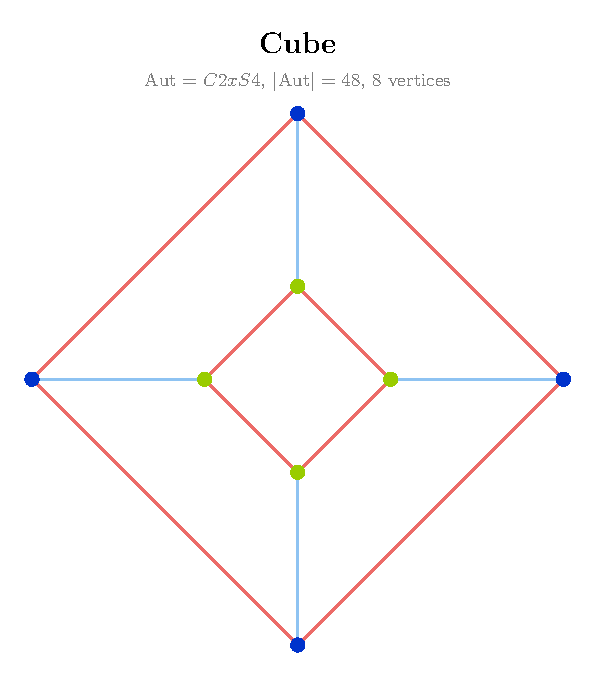
\includegraphics[width=\textwidth]{auto-cube.pdf}
  \caption{Cube}
\end{subfigure}\hfill
\begin{subfigure}[b]{0.24\textwidth}
  \centering
  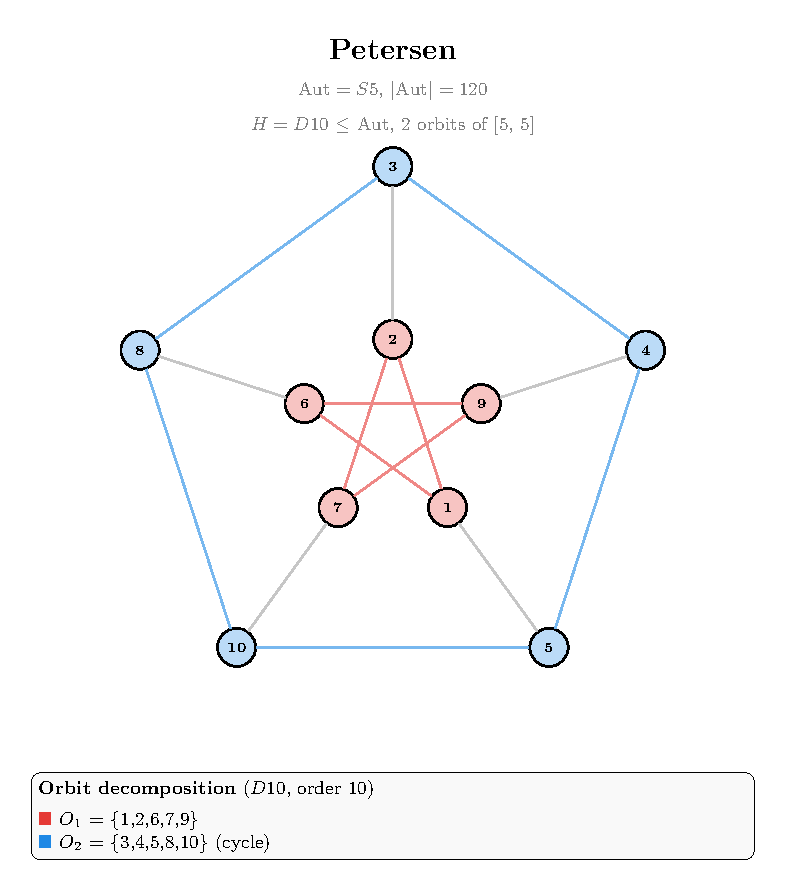
\includegraphics[width=\textwidth]{auto-petersen.pdf}
  \caption{Petersen}
\end{subfigure}\hfill
\begin{subfigure}[b]{0.24\textwidth}
  \centering
  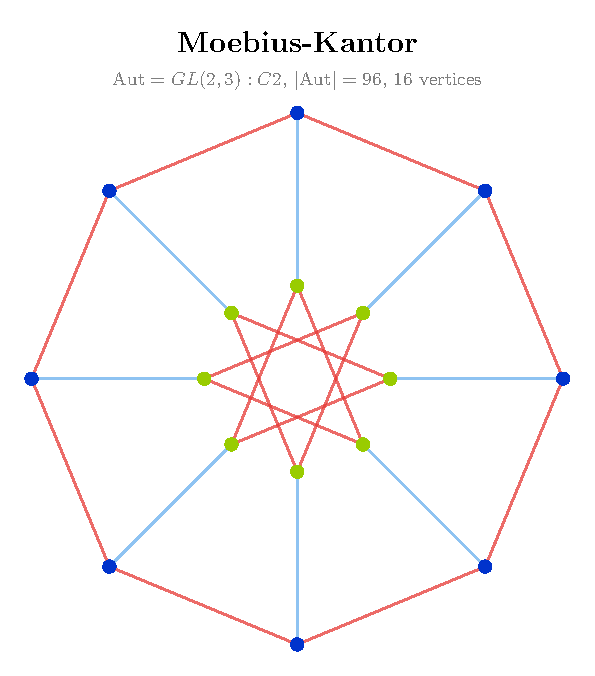
\includegraphics[width=\textwidth]{auto-moebiuskantor.pdf}
  \caption{M\"obius-Kantor}
\end{subfigure}\hfill
\begin{subfigure}[b]{0.24\textwidth}
  \centering
  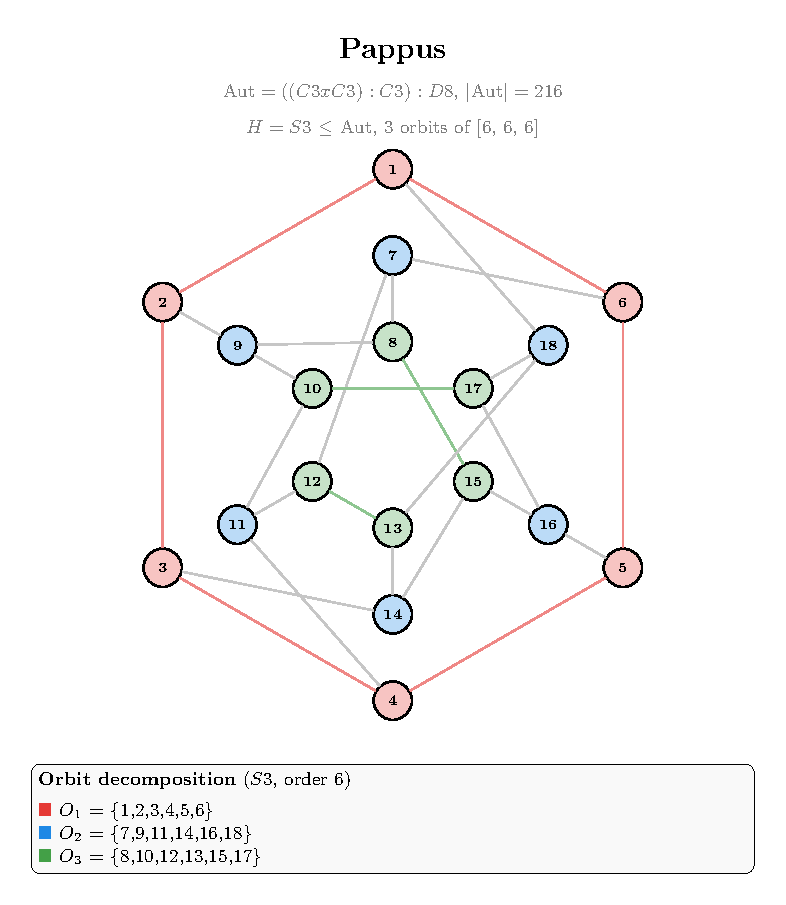
\includegraphics[width=\textwidth]{auto-pappus.pdf}
  \caption{Pappus}
\end{subfigure}

\medskip
\begin{subfigure}[b]{0.24\textwidth}
  \centering
  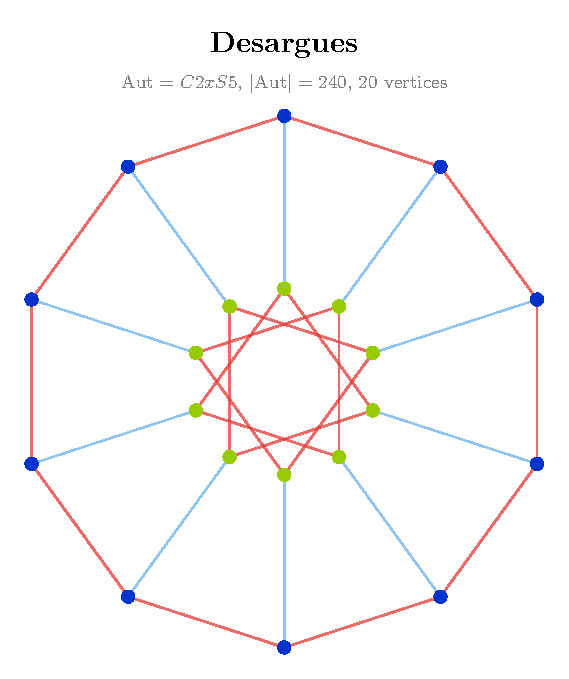
\includegraphics[width=\textwidth]{auto-desargues.pdf}
  \caption{Desargues}
\end{subfigure}\hfill
\begin{subfigure}[b]{0.24\textwidth}
  \centering
  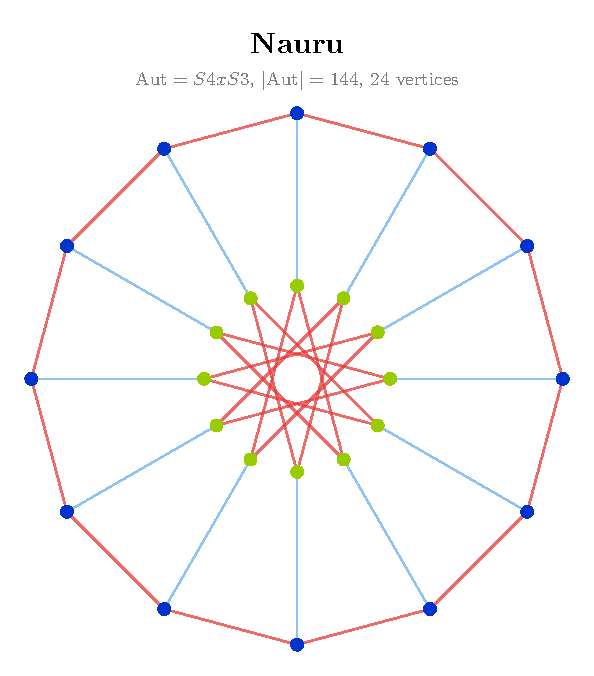
\includegraphics[width=\textwidth]{auto-nauru.pdf}
  \caption{Nauru}
\end{subfigure}\hfill
\begin{subfigure}[b]{0.24\textwidth}
  \centering
  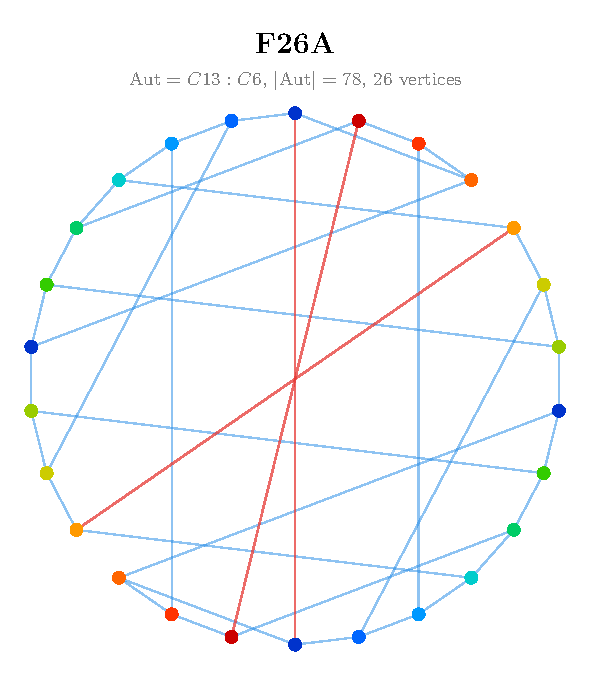
\includegraphics[width=\textwidth]{auto-f26a.pdf}
  \caption{F26A}
\end{subfigure}\hfill
\begin{subfigure}[b]{0.24\textwidth}
  \centering
  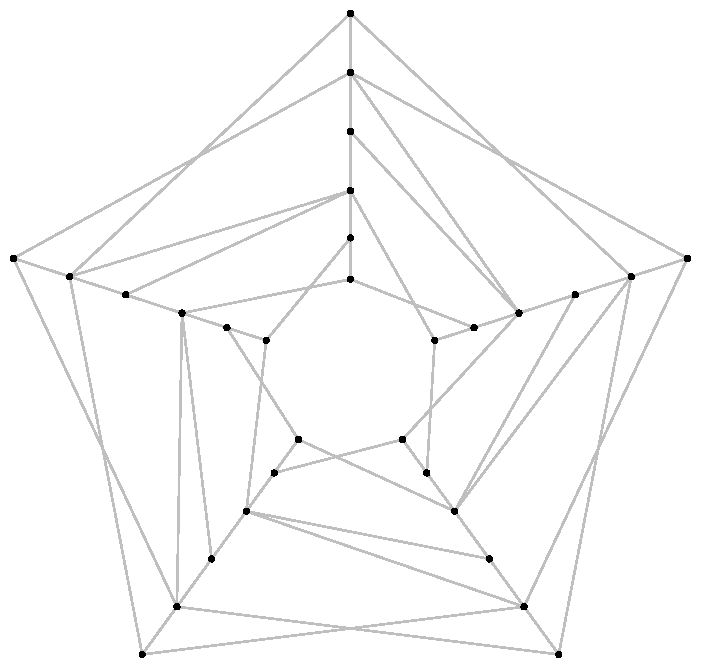
\includegraphics[width=\textwidth]{tuttecoxeter-clean.pdf}
  \caption{Tutte-Coxeter}
\end{subfigure}
\caption{Eight Foster census graphs. The layout algorithm places vertices on
  concentric rings respecting the orbit structure of a chosen quotient
  subgroup, minimising edge crossings.}
\label{fig:foster}
\end{figure}


% ==========================================================================
\section{Graph constructions and census}
% ==========================================================================

Each graph in the census up to 30 vertices belongs to one of two natural
families: generalised Petersen graphs $\GP(n,k)$ or LCF graphs, with
a few ad hoc constructions (the dodecahedron, Coxeter graph, $K_4$,
$K_{3,3}$).

\begin{tcolorbox}[breakable, colback=black!5, colframe=black!5,
  boxrule=0pt, sharp corners]
\centering
\captionof{table}{Foster census cubic arc-transitive graphs up to 30 vertices.}
\label{tab:census}
\small
\begin{tabular}{llrrrrl}
\toprule
Graph & Foster label & $n$ & Girth & Diam.\ & $|\Aut|$ & Construction \\
\midrule
$K_4$             & F004   &  4 & 3 & 1 & 24    & Complete graph \\
$K_{3,3}$         & F006   &  6 & 4 & 2 & 72    & Complete bipartite \\
Cube              & F008   &  8 & 4 & 3 & 48    & $\GP(4,1)$ \\
Petersen          & F010   & 10 & 5 & 2 & 120   & $\GP(5,2)$ \\
Heawood           & F014   & 14 & 6 & 3 & 336   & $\mathrm{LCF}[5,-5]^7$ \\
M\"{o}bius--Kantor & F016   & 16 & 6 & 4 & 96    & $\GP(8,3)$ \\
Pappus            & F018   & 18 & 6 & 4 & 216   & $\mathrm{LCF}[5,7,-7,7,-7,-5]^3$ \\
Dodecahedron      & F020A  & 20 & 5 & 5 & 120   & Platonic solid \\
Desargues         & F020B  & 20 & 6 & 5 & 240   & $\GP(10,3)$ \\
Nauru             & F024   & 24 & 6 & 4 & 144   & $\GP(12,5)$ \\
F26A              & F026A  & 26 & 6 & 5 & 78    & $\mathrm{LCF}[-7,7]^{13}$ \\
Coxeter           & F028   & 28 & 7 & 4 & 336   & Hub + three 7-cycles \\
Tutte--Coxeter    & F030   & 30 & 8 & 4 & 1440  & $\mathrm{LCF}[-13,-9,7,-7,9,13]^5$ \\
\bottomrule
\end{tabular}
\end{tcolorbox}


% ==========================================================================
\section{Spectral results}
% ==========================================================================

\begin{tcolorbox}[breakable, colback=black!5, colframe=black!5,
  boxrule=0pt, sharp corners]
\centering
\captionof{table}{Adjacency spectral data for Foster census graphs (all cubic, $\lambda_1 = 3$).
Refer to the master table (Table~\ref{tab:master}) for cross-family comparison.}
\label{tab:spectra-foster}
\small
\begin{tabular}{lrrrrrcccc}
\toprule
Graph & $\lambda_2$ & $\lambda_{\min}$ & Gap & Fiedler & \#dist. & Bip.\ & Ram.\ & DT \\
\midrule
$K_4$             & $-1$        & $-1$       & $4$      & $4$      & 2 & N & Y & Y \\
$K_{3,3}$         & $0$         & $-3$       & $3$      & $3$      & 3 & Y & Y & Y \\
Cube              & $1$         & $-3$       & $2$      & $2$      & 4 & Y & Y & Y \\
Petersen          & $1$         & $-2$       & $2$      & $2$      & 3 & N & Y & Y \\
Heawood           & $\sqrt{2}$  & $-3$       & $3-\sqrt{2}$ & $3-\sqrt{2}$ & 4 & Y & Y & Y \\
M\"{o}b.--Kant. & $\sqrt{3}$  & $-3$       & $3-\sqrt{3}$ & $3-\sqrt{3}$ & 6 & Y & Y & N \\
Pappus            & $\sqrt{3}$  & $-3$       & $3-\sqrt{3}$ & $3-\sqrt{3}$ & 5 & Y & Y & Y \\
Dodecahedron      & $\frac{1+\sqrt{5}}{2}$ & $-\frac{1+\sqrt{5}}{2}$ & $\frac{5-\sqrt{5}}{2}$ & $\frac{5-\sqrt{5}}{2}$ & 6 & N & Y & Y \\
Desargues         & $2$         & $-3$       & $1$      & $1$      & 6 & Y & Y & Y \\
Nauru             & $2$         & $-3$       & $1$      & $1$      & 7 & Y & Y & N \\
F26A              & $\beta$     & $-3$       & $3-\beta$ & $3-\beta$ & 6 & Y & Y & Y \\
Coxeter           & $2$         & $-1-\sqrt{2}$ & $1$  & $1$      & 5 & N & Y & Y \\
Tutte--Coxeter    & $2$         & $-3$       & $1$      & $1$      & 5 & Y & Y & Y \\
\bottomrule
\multicolumn{9}{l}{\small $\beta = \sqrt{(5+\sqrt{13})/2} \approx 2.074$; Bip.\ = bipartite; Ram.\ = Ramanujan; DT = distance-transitive.}
\end{tabular}
\end{tcolorbox}


\subsection{Complete eigenvalue spectra}

We list the complete spectrum $\{(\lambda, \text{mult})\}$ for each graph.
Spectra of bipartite graphs are symmetric about~0.

\medskip
\noindent
$K_4$: $\{(3, 1),\; (-1, 3)\}$. \quad
$K_{3,3}$: $\{(3, 1),\; (0, 4),\; (-3, 1)\}$.

\medskip
\noindent
\textbf{Cube}: $\{(3,1),\; (1,3),\; (-1,3),\; (-3,1)\}$. This is the $Q_3$ hypercube; all eigenvalues are integers.

\medskip
\noindent
\textbf{Petersen}: $\{(3,1),\; (1,5),\; (-2,4)\}$. The Petersen graph is the Kneser graph $K(5,2)$; its eigenvalues are $3$, $1$, and $-2$.

\medskip
\noindent
\textbf{Heawood}: $\{(3,1),\; (\sqrt{2},6),\; (-\sqrt{2},6),\; (-3,1)\}$. The Heawood graph is the incidence graph of the Fano plane $\mathrm{PG}(2,2)$. It reappears in Part~V as the voltage lift $\CR(7)$.

\medskip
\noindent
\textbf{M\"{o}bius--Kantor} $(\GP(8,3))$: $\{(3,1),\; (\sqrt{3},4),\; (1,3),\; (-1,3),\; (-\sqrt{3},4),\; (-3,1)\}$. Six distinct eigenvalues but diameter~4: this is the only graph in the census with $|\mathrm{spec}| \neq \mathrm{diam}+1$ that is bipartite.

\medskip
\noindent
\textbf{Pappus}: $\{(3,1),\; (\sqrt{3},6),\; (0,4),\; (-\sqrt{3},6),\; (-3,1)\}$. The zero eigenvalue has multiplicity~4, reflecting the graph's triangle-free nature.

\medskip
\noindent
\textbf{Dodecahedron}: $\{(3,1),\; (\phi,3),\; (1,5),\; (0,4),\; (-2,4),\; (-\phi,3)\}$ where $\phi = \tfrac{1+\sqrt{5}}{2}$. The spectrum reflects icosahedral ($A_5$) symmetry.

\medskip
\noindent
\textbf{Desargues} $(\GP(10,3))$: $\{(3,1),\; (2,4),\; (1,5),\; (-1,5),\; (-2,4),\; (-3,1)\}$. Bipartite and distance-transitive with all integer eigenvalues.

\medskip
\noindent
\textbf{Nauru} $(\GP(12,5))$: $\{(3,1),\; (2,6),\; (1,3),\; (0,4),\; (-1,3),\; (-2,6),\; (-3,1)\}$. Seven distinct eigenvalues; diameter~4 gives $4+1=5 \neq 7$, so Nauru is \emph{not} distance-transitive.

\medskip
\noindent
\textbf{F26A} $(\mathrm{LCF}[-7,7]^{13})$: $\{(3,1),\; (\beta,6),\; (\alpha,6),\; (-\alpha,6),\; (-\beta,6),\; (-3,1)\}$
where $\beta = \sqrt{(5+\sqrt{13})/2} \approx 2.074$, $\alpha = \sqrt{(5-\sqrt{13})/2} \approx 0.835$.
The discriminant~13 matches the $\Z_{13}$ symmetry. This graph reappears in Part~V as $\CR(13)$.

\medskip
\noindent
\textbf{Coxeter}: $\{(3,1),\; (2,8),\; (\sqrt{2}-1,6),\; (-1,7),\; (-1-\sqrt{2},6)\}$.
The unique non-Hamiltonian cubic distance-transitive graph.

\medskip
\noindent
\textbf{Tutte--Coxeter} (Levi graph of $\mathrm{GQ}(2,2)$): $\{(3,1),\; (2,9),\; (0,10),\; (-2,9),\; (-3,1)\}$. All eigenvalues are integers.


\subsection{Discussion}

\begin{tcolorbox}[breakable, colback=yellow!10, colframe=yellow!10,
  boxrule=0pt, sharp corners]
\textbf{Key findings from the Foster census:}
\begin{enumerate}[noitemsep]
\item Every graph is Ramanujan.
\item Eleven of the thirteen are distance-transitive; the exceptions are $\GP(8,3)$ and $\GP(12,5)$.
\item The spectral gap decreases with graph order, with the Dodecahedron as an outlier (smallest gap despite only 20 vertices).
\item The algebraic fields generated by eigenvalues are $\Q$, $\Q(\sqrt{2})$, $\Q(\sqrt{3})$, $\Q(\sqrt{5})$, and $\Q(\sqrt{13})$, all arising from the prime structure of symmetry groups.
\item Four graphs share the gap value $1$: Desargues, Nauru, Coxeter, and Tutte--Coxeter. All have $\lambda_2 = 2$.
\end{enumerate}

These observations motivate the central question: as one moves to larger arc-transitive graphs, does arc-transitivity force spectral gaps to stay bounded away from the Ramanujan threshold? The $\PSL(2,q)$ family (Part~III) provides a natural infinite sequence to test this.
\end{tcolorbox}


% ======================================================================
%
%  PART III: THE SU(2) FAMILY
%
% ======================================================================

\newpage
\part*{Part III: The SU(2) Family}
\addcontentsline{toc}{part}{Part III: The SU(2) Family --- $\PSL(2,q)$}

% ==========================================================================
\section{The three PSL(2,q) families}
% ==========================================================================

For $G = \PSL(2,\F_q)$ (with $q$ an odd prime power), the subgroup structure
yields exactly three families of cubic arc-transitive Sabidussi graphs,
parametrised by $H \in \{C_3, S_3, S_4\}$. These graphs may be regarded as
finite shadows of the infinite cubic tree on which
$\SU(2,\C)$ acts, hence the designation ``SU(2) cubic graphs.''

\begin{tcolorbox}[colback=black!5, colframe=black!5,
  boxrule=0pt, sharp corners]
\begin{center}
\begin{tabular}{llll}
\toprule
Family & $H$ & $|H|$ & $|V| = |G|/|H|$ \\
\midrule
$C_3$ & cyclic of order 3 & 3 & $q(q^2-1)/6$ \\
$S_3$ & symmetric group & 6 & $q(q^2-1)/12$ \\
$S_4$ & symmetric group & 24 & $q(q^2-1)/48$ \\
\bottomrule
\end{tabular}
\end{center}
The inclusions $C_3 \subset S_3 \subset S_4$ give a tower of quotient maps
$\Gamma(G, C_3) \twoheadrightarrow \Gamma(G, S_3) \twoheadrightarrow \Gamma(G, S_4)$,
with spectral nesting discussed in Section~\ref{sec:nesting-psl}.
\end{tcolorbox}

\begin{figure}[ht]
\centering
\begin{subfigure}[b]{0.48\textwidth}
  \centering
  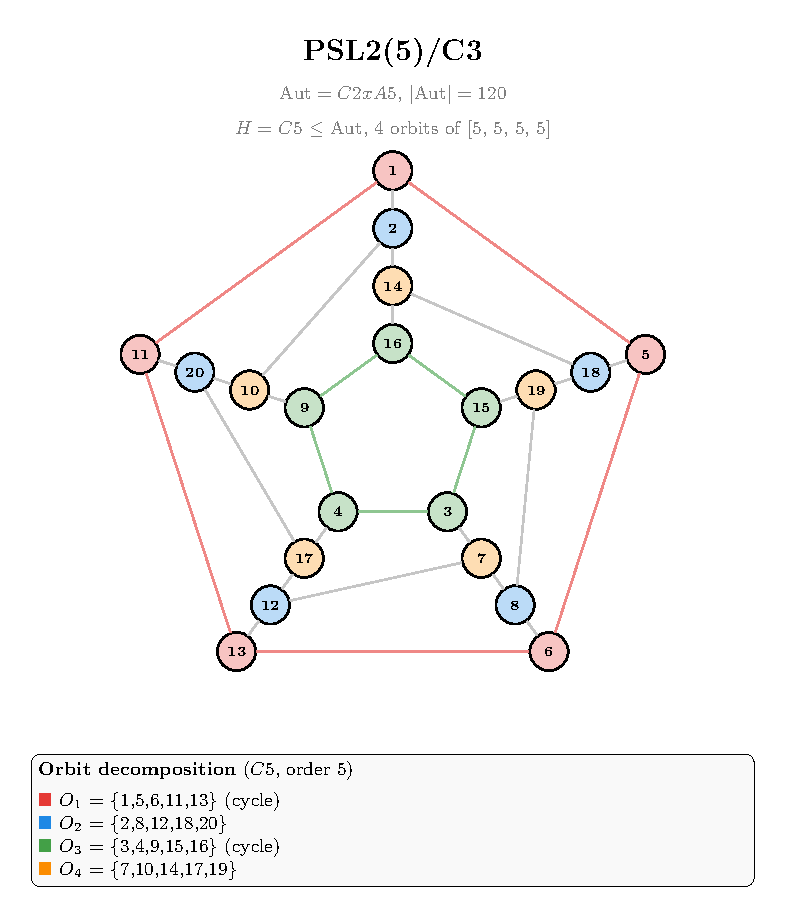
\includegraphics[width=\textwidth]{auto-psl2_5_c3.pdf}
  \caption{$\Sab(\PSL(2,5), C_3)$: the icosahedron (20 vertices).}
\end{subfigure}
\hfill
\begin{subfigure}[b]{0.48\textwidth}
  \centering
  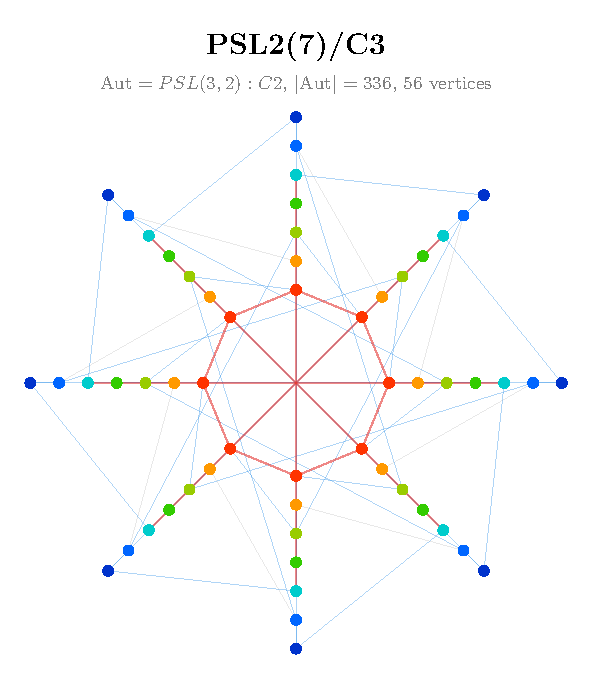
\includegraphics[width=\textwidth]{auto-psl2_7_c3.pdf}
  \caption{$\Sab(\PSL(2,7), C_3)$: the Klein graph (56 vertices).}
\end{subfigure}

\medskip

\begin{subfigure}[b]{0.48\textwidth}
  \centering
  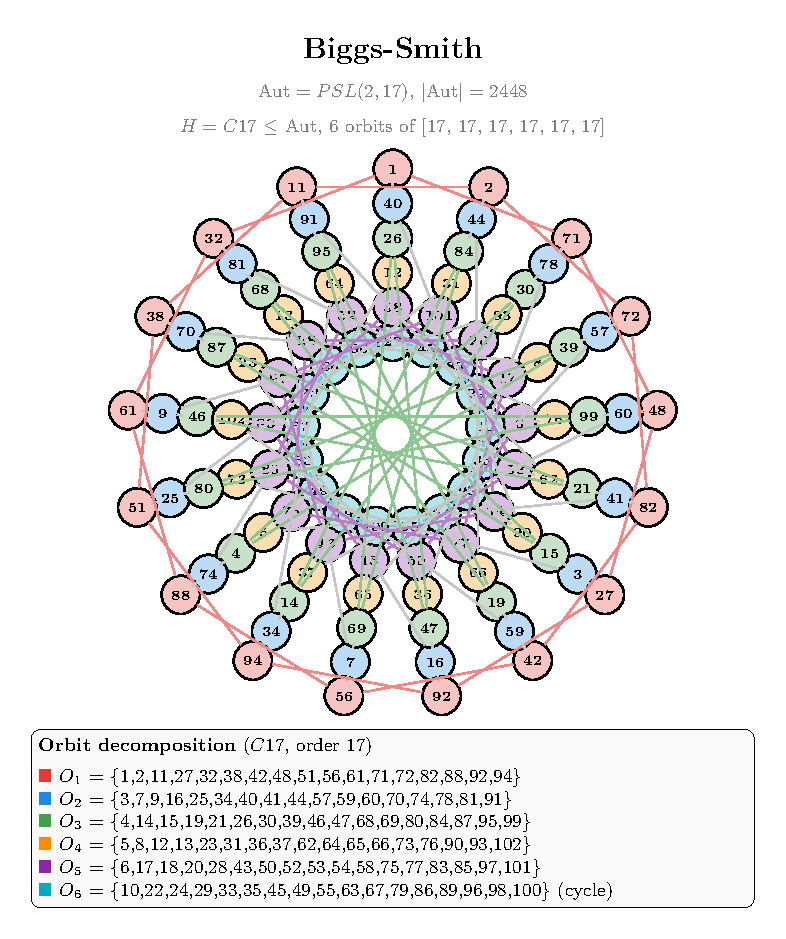
\includegraphics[width=\textwidth]{auto-biggssmith.pdf}
  \caption{The Biggs--Smith graph $\Sab(\PSL(2,17), S_4)$ (102 vertices).}
\end{subfigure}
\hfill
\begin{subfigure}[b]{0.48\textwidth}
  \centering
  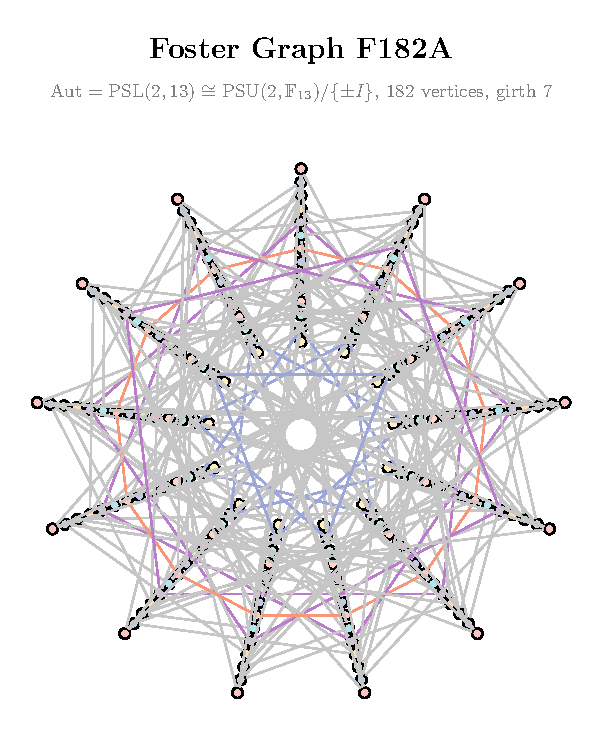
\includegraphics[width=\textwidth]{auto-psl2_13.pdf}
  \caption{$\Sab(\PSL(2,13), S_3)$: 182 vertices.}
\end{subfigure}
\caption{Representative graphs from the three PSL$(2,q)$ families, drawn with
  symmetry-aware orbit quotient layouts. The rotational symmetry reflects the
  cyclic structure of the chosen orbit decomposition.}
\label{fig:psl2-graphs}
\end{figure}

\subsection{Census of graphs}

\begin{tcolorbox}[colback=black!5, colframe=black!5,
  boxrule=0pt, sharp corners]
\begin{center}
\begin{tabular}{llllc}
\toprule
Graph & $q$ & $H$ & $|V|$ & Common name \\
\midrule
$\Sab(\PSL(2,\F_5), C_3, \cdot)$ & 5 & $C_3$ & 20 & (double cover of Petersen) \\
$\Sab(\PSL(2,\F_5), S_3, \cdot)$ & 5 & $S_3$ & 10 & Petersen graph \\
$\Sab(\PSL(2,\F_7), C_3, \cdot)$ & 7 & $C_3$ & 56 & Klein graph $F_{056}A$ \\
$\Sab(\PSL(2,\F_{11}), C_3, \cdot)$ & 11 & $C_3$ & 220 & --- \\
$\Sab(\PSL(2,\F_{13}), S_3, \cdot)$ & 13 & $S_3$ & 182 & --- \\
$\Sab(\PSL(2,\F_{17}), S_3, \cdot)$ & 17 & $S_3$ & 408 & --- \\
$\Sab(\PSL(2,\F_{17}), S_4, \cdot)$ & 17 & $S_4$ & 102 & Biggs-Smith graph \\
\bottomrule
\end{tabular}
\end{center}
\end{tcolorbox}


% ==========================================================================
\section{Spectral data}
% ==========================================================================

\subsection{Summary table}

\begin{tcolorbox}[breakable, colback=black!5, colframe=black!5,
  boxrule=0pt, sharp corners]
\captionof{table}{Key spectral properties of the SU(2) cubic Sabidussi family.
The Ramanujan bound is $2\sqrt{2} \approx 2.828$.
Cross-reference with the master table (Table~\ref{tab:master}).}
\label{tab:summary-psl}
\begin{center}
\begin{tabular}{lrllrrrrrc}
\toprule
Graph & $q$ & $H$ & $|V|$ & $g$ & $\lambda_2$ & $\mu_1$ & $\lambda_1 - \lambda_2$ & $\#\lambda$ & Ram? \\
\midrule
$\PSL(2,5)/C_3$  &  5 & $C_3$ &  20 & 5 & $2.236$ & $0.764$ & $0.764$ &  6 & \checkmark \\
Petersen                  &  5 & $S_3$ &  10 & 5 & $1.000$ & $2.000$ & $2.000$ &  3 & \checkmark \\
Klein $F_{056}A$          &  7 & $C_3$ &  56 & 6 & $2.414$ & $0.586$ & $0.586$ &  9 & \checkmark \\
$\PSL(2,11)/C_3$ & 11 & $C_3$ & 220 & 10 & $2.618$ & $0.382$ & $0.382$ & 19 & \checkmark \\
$\PSL(2,13)/S_3$ & 13 & $S_3$ & 182 & 7 & $2.675$ & $0.325$ & $0.325$ & 16 & \checkmark \\
Biggs-Smith               & 17 & $S_4$ & 102 & 9 & $2.562$ & $0.438$ & $0.438$ &  8 & \checkmark \\
$\PSL(2,17)/S_3$ & 17 & $S_3$ & 408 & 9 & $2.709$ & $0.291$ & $0.291$ & 24 & \checkmark \\
\bottomrule
\end{tabular}
\end{center}
\end{tcolorbox}


\subsection{Full spectra}

\begin{tcolorbox}[breakable, colback=black!5, colframe=black!5,
  boxrule=0pt, sharp corners]

\noindent\textbf{PSL(2,5)/C$_3$} \quad ($n=20$, girth~5)
\smallskip

\begin{center}
\begin{tabular}{rrl}
\toprule
Eigenvalue & Mult. & Algebraic form \\
\midrule
$3.000$ & 1 & $3$ \\
$2.236$ & 3 & $\sqrt{5}$ \\
$1.000$ & 5 & $1$ \\
$0.000$ & 4 & $0$ \\
$-2.000$ & 4 & $-2$ \\
$-2.236$ & 3 & $-\sqrt{5}$ \\
\bottomrule
\end{tabular}
\end{center}

\bigskip\noindent\textbf{PSL(2,5)/S$_3$ = Petersen graph} \quad ($n=10$, girth~5)
\smallskip

\begin{center}
\begin{tabular}{rrl}
\toprule
Eigenvalue & Mult. & Algebraic form \\
\midrule
$3.000$ & 1 & $3$ \\
$1.000$ & 5 & $1$ \\
$-2.000$ & 4 & $-2$ \\
\bottomrule
\end{tabular}
\end{center}

\bigskip\noindent\textbf{PSL(2,7)/C$_3$ = Klein graph $F_{056}A$} \quad ($n=56$, girth~6)
\smallskip

\begin{center}
\begin{tabular}{rrl}
\toprule
Eigenvalue & Mult. & Algebraic form \\
\midrule
$3.000$ & 1 & $3$ \\
$2.414$ & 8 & $1+\sqrt{2}$ \\
$1.562$ & 7 & (root of $x^3 - 3x - 1 = 0$ over $\Q(\cos(2\pi/7))$) \\
$1.414$ & 6 & $\sqrt{2}$ \\
$0.000$ & 7 & $0$ \\
$-0.414$ & 8 & $1-\sqrt{2}$ \\
$-1.414$ & 6 & $-\sqrt{2}$ \\
$-2.000$ & 6 & $-2$ \\
$-2.562$ & 7 & \\
\bottomrule
\end{tabular}
\end{center}

\bigskip\noindent\textbf{PSL(2,11)/C$_3$} \quad ($n=220$, girth~10)
\smallskip

\begin{center}
\begin{tabular}{rrl}
\toprule
Eigenvalue & Mult. & Algebraic form \\
\midrule
$3.000$ & 1 & $3$ \\
$2.618$ & 12 & $(3+\sqrt{5})/2$ \\
$2.497$ & 12 & \\
$2.175$ & 10 & \\
$2.000$ & 11 & $2$ \\
$1.618$ & 12 & $(1+\sqrt{5})/2 = \phi$ \\
$1.328$ & 12 & \\
$1.126$ & 10 & \\
$0.732$ & 10 & $-1+\sqrt{3}$ \\
$0.382$ & 12 & $(3-\sqrt{5})/2$ \\
$0.000$ & 20 & $0$ \\
$-0.618$ & 12 & $(1-\sqrt{5})/2$ \\
$-1.000$ & 11 & $-1$ \\
$-1.126$ & 10 & \\
$-1.328$ & 12 & \\
$-2.000$ & 21 & $-2$ \\
$-2.175$ & 10 & \\
$-2.497$ & 12 & \\
$-2.732$ & 10 & $-1-\sqrt{3}$ \\
\bottomrule
\end{tabular}
\end{center}

\bigskip\noindent\textbf{PSL(2,13)/S$_3$} \quad ($n=182$, girth~7)
\smallskip

\begin{center}
\begin{tabular}{rrl}
\toprule
Eigenvalue & Mult. & Algebraic form \\
\midrule
$3.000$ & 1 & $3$ \\
$2.675$ & 14 & \\
$2.115$ & 13 & \\
$1.987$ & 12 & \\
$1.539$ & 14 & \\
$1.303$ & 7 & \\
$1.086$ & 12 & \\
$0.257$ & 12 & \\
$-0.254$ & 13 & \\
$-0.284$ & 12 & \\
$-1.000$ & 14 & $-1$ \\
$-1.214$ & 14 & \\
$-1.861$ & 13 & \\
$-2.303$ & 7 & \\
$-2.504$ & 12 & \\
$-2.542$ & 12 & \\
\bottomrule
\end{tabular}
\end{center}

\bigskip\noindent\textbf{PSL(2,17)/S$_4$ = Biggs-Smith graph} \quad ($n=102$, girth~9)
\smallskip

\begin{center}
\begin{tabular}{rrl}
\toprule
Eigenvalue & Mult. & Algebraic form \\
\midrule
$3.000$ & 1 & $3$ \\
$2.562$ & 9 & \\
$2.000$ & 18 & $2$ \\
$0.879$ & 16 & \\
$0.000$ & 17 & $0$ \\
$-1.347$ & 16 & \\
$-1.562$ & 9 & \\
$-2.532$ & 16 & \\
\bottomrule
\end{tabular}
\end{center}

\bigskip\noindent\textbf{PSL(2,17)/S$_3$} \quad ($n=408$, girth~9)
\smallskip

\begin{center}
\begin{tabular}{rrl}
\toprule
Eigenvalue & Mult. & Algebraic form \\
\midrule
$3.000$ & 1 & $3$ \\
$2.709$ & 18 & \\
$2.562$ & 9 & \\
$2.373$ & 16 & \\
$2.236$ & 17 & $\sqrt{5}$ \\
$2.000$ & 18 & $2$ \\
$1.965$ & 16 & \\
$1.414$ & 34 & $\sqrt{2}$ \\
$1.000$ & 18 & $1$ \\
$0.879$ & 16 & \\
$0.414$ & 18 & $\sqrt{2}-1$ \\
$0.194$ & 18 & \\
$0.000$ & 17 & $0$ \\
$-0.146$ & 16 & \\
$-0.691$ & 16 & \\
$-0.780$ & 16 & \\
$-1.347$ & 16 & \\
$-1.414$ & 34 & $-\sqrt{2}$ \\
$-1.562$ & 9 & \\
$-1.903$ & 18 & \\
$-2.236$ & 17 & $-\sqrt{5}$ \\
$-2.414$ & 18 & $-(1+\sqrt{2})$ \\
$-2.532$ & 16 & \\
$-2.721$ & 16 & \\
\bottomrule
\end{tabular}
\end{center}
\end{tcolorbox}


% ==========================================================================
\section{All graphs are Ramanujan}
% ==========================================================================

\begin{tcolorbox}[colback=black!5, colframe=black!5,
  boxrule=0pt, sharp corners]
\begin{theorem}\label{thm:all_ram}
Every graph in the SU(2) cubic Sabidussi family is Ramanujan: for each graph
$\Gamma$ above, $\lambda_2(\Gamma) \leq 2\sqrt{2}$.
\end{theorem}
\end{tcolorbox}

The tightest bound is achieved by $\PSL(2,17)/S_3$ with
$\lambda_2 \approx 2.709$, well below $2\sqrt{2} \approx 2.828$.

\begin{tcolorbox}[breakable, colback=yellow!10, colframe=yellow!10,
  boxrule=0pt, sharp corners]
\textbf{Connection to the Ramanujan--Petersson conjecture.}
The adjacency operator on $\ell^2(G/H)$ decomposes as a direct sum over
irreducible representations $\pi$ of $G$ that contain the trivial
$H$-type (spherical representations). The eigenvalue associated to $\pi$
is the \emph{Hecke eigenvalue}
\[
  \lambda_\pi = \frac{\mu(HaH)}{\mu(H)}\,\hat{\phi}(\pi),
\]
where $\hat\phi(\pi)$ is the spherical transform of the indicator function
of the double coset $HaH$.

The Ramanujan condition $|\lambda_\pi| \leq 2\sqrt{k-1}$ for all
non-trivial spherical representations is precisely the content of the
Ramanujan--Petersson conjecture for the Hecke algebra $\mathcal{H}(G,H)$.
For $G = \PSL(2,\F_q)$, this reduces to bounds on Kloosterman sums and
character sums over $\F_q$, controlled by Weil's theorem~\cite{Weil}.
\end{tcolorbox}


% ==========================================================================
\section{Algebraic eigenvalues}
% ==========================================================================

\begin{tcolorbox}[colback=yellow!10, colframe=yellow!10,
  boxrule=0pt, sharp corners]
\textbf{Golden ratio in PSL(2,11)/C$_3$.}
The golden ratio $\phi = (1+\sqrt{5})/2$ occurs with multiplicity~12,
as does $1+\phi = (3+\sqrt{5})/2$. This arises because $\PSL(2,\F_{11})$
has character degrees divisible by~5, and the 5th cyclotomic field
$\Q(\zeta_5)$ contains $\sqrt{5}$.
\end{tcolorbox}

\begin{tcolorbox}[colback=yellow!10, colframe=yellow!10,
  boxrule=0pt, sharp corners]
\textbf{$\sqrt{2}$ in Klein and Biggs-Smith.}
The Klein graph has $\lambda_2 = 1+\sqrt{2}$ (multiplicity~8) because the
Hecke algebra $\mathcal{H}(\PSL(2,\F_7), C_3)$ has a 2-dimensional block
with characteristic polynomial $x^2 - 2x - 1 = 0$, giving roots $1\pm\sqrt{2}$.
The same algebraic numbers appear prominently in $\PSL(2,17)/S_3$, where
$\sqrt{2}$ has multiplicity~34.
\end{tcolorbox}

The Biggs-Smith graph is the only distance-regular graph in the family.
Its 8 distinct eigenvalues match $\text{diameter} + 1 = 8$, and they are
the eigenvalues of the intersection array
$\{3,2,2,2,1,1,1;\, 1,1,1,1,1,1,3\}$~\cite{BCN}. The characteristic
polynomial factors over $\Q(\sqrt{2}, \sqrt{17})$.


% ==========================================================================
\section{Fiedler eigenvalue and the Biggs-Smith anomaly}
% ==========================================================================

\begin{tcolorbox}[colback=black!5, colframe=black!5,
  boxrule=0pt, sharp corners]
The Fiedler scaling $\mu_1 \approx 4/q$ for the $C_3$ family was
presented in the synthesis (Proposition~\ref{prop:fiedler-A1}).

The Biggs-Smith graph ($q=17$, $H=S_4$, $n=102$) has a substantially
larger Fiedler eigenvalue ($\mu_1 \approx 0.438$) than the 408-vertex
$S_3$-graph at the same prime ($\mu_1 \approx 0.291$). This is the
\emph{tightness} effect: the larger stabiliser $S_4$ collapses 4 times
as many orbits, yielding a smaller graph with a wider spectral gap.
\end{tcolorbox}


% ==========================================================================
\section{Spectral nesting at $q = 17$}
\label{sec:nesting-psl}
% ==========================================================================

The chain $C_3 \subset S_3 \subset S_4$ induces covering maps between
Sabidussi graphs. Each covering map induces spectral containment.

At $q=17$, the Biggs-Smith graph has 8 distinct eigenvalues:
$\{3, 2.562, 2, 0.879, 0, -1.347, -1.562, -2.532\}$.
All eight appear in the spectrum of the 408-vertex $\PSL(2,17)/S_3$ graph.
The 16 ``new'' eigenvalues in the $S_3$ graph arise from representations
of $\PSL(2,17)$ that factor through $S_3$ but not through $S_4$.


% ==========================================================================
\section{Representation-theoretic interpretation}
% ==========================================================================

\begin{tcolorbox}[breakable, colback=yellow!10, colframe=yellow!10,
  boxrule=0pt, sharp corners]
\textbf{Hecke algebras and spherical functions.}
The \emph{Hecke algebra} $\mathcal{H}(G,H)$ is the convolution algebra of
$H$-biinvariant functions on $G$. Its one-dimensional representations are
the \emph{spherical functions} $\omega_\pi\colon G \to \C$, indexed by the
irreducible representations $\pi$ of $G$ containing the trivial $H$-type.
The adjacency eigenvalues of $\Sab(G,H,HaH)$ are exactly:
\[
  \lambda_\pi = \omega_\pi(a) =
    \frac{1}{|H|} \sum_{g \in HaH} \chi_\pi(g)/d_\pi,
\]
where $\chi_\pi$ is the character and $d_\pi = \dim\pi$.
The multiplicity of $\lambda_\pi$ equals the dimension of the $H$-fixed
space in $\pi$, by Frobenius reciprocity.
\end{tcolorbox}

\begin{tcolorbox}[breakable, colback=blue!5, colframe=blue!5,
  boxrule=0pt, sharp corners]
\textbf{Open questions.}
\begin{itemize}[noitemsep]
\item \textbf{$C_3$ family beyond $q=11$.} The next graph would be
  $\PSL(2,13)/C_3$ (364 vertices). Based on the trend, we expect
  $\lambda_2 \to 3^-$ with $\mu_1 \approx 4/q$.
\item \textbf{Algebraic degrees.} For $\PSL(2,q)/C_3$, $\lambda_2$ has
  algebraic degree~2 for $q = 5, 7, 11$. Does degree~2 persist for all~$q$?
\item \textbf{Non-split extensions.} The groups $\PGL(2,\F_q)$ also act on
  related Cayley graphs; their spectra may involve non-tempered
  representations.
\end{itemize}
\end{tcolorbox}


% ======================================================================
%
%  PART IV: THE EXCEPTIONAL LIE GROUP G_2(2)
%
% ======================================================================

\newpage
\part*{Part IV: The Exceptional Lie Group $G_2(2)$}
\addcontentsline{toc}{part}{Part IV: The Exceptional Lie Group $G_2(2)$}

% ==========================================================================
\section{The group $G_2(2)$ and split octonions}
% ==========================================================================

The split octonion algebra $\mathbb{O}'$ over $\F_2$ is an 8-dimensional
algebra with a non-degenerate quadratic form of Witt index~4. Its automorphism
group is the exceptional algebraic group $G_2$, yielding the finite group
$G_2(2)$ of order
\[
  |G_2(2)| = 2^6 \cdot 3^3 \cdot 7 = 12096.
\]
The derived subgroup $G_2(2)'$ is $\PSU(3,3)$ of order 6048, a simple group.

\subsection{The split Cayley hexagon $\GH$}

A \emph{generalized hexagon of order $(s,t)$} is a point-line geometry whose
incidence graph has girth~12. The split Cayley hexagon $\GH$ has $s = t = 2$,
giving 63 points, 63 lines, each point on 3 lines, each line through 3 points.
The full automorphism group of $\GH$ is $G_2(2)$.


% ==========================================================================
\section{The three graphs}
% ==========================================================================

\begin{tcolorbox}[colback=green!8, colframe=green!8,
  boxrule=0pt, sharp corners]
\begin{definition}
The \emph{Tutte 12-cage} is the point-line incidence graph of $\GH$: 126
vertices (63 points + 63 lines), 3-regular, girth~12. It is the unique
$(3,12)$-cage and is distance-transitive with diameter~6.
\end{definition}

\begin{definition}
The \emph{$\GH$ collinearity graph} is the graph on the 63 points of $\GH$
where two points are adjacent iff collinear. It is 6-regular, distance-regular
with intersection array $\{6,4,4;1,1,3\}$.
\end{definition}

\begin{definition}
The \emph{Meinhold-72 graph} is a quotient of the Clayworth graph by
$K = \PSL(3,2) \cong \PSL(2,7)$. It has 72 vertices, is 7-regular, girth~4,
diameter~5, and is not distance-regular.
\end{definition}
\end{tcolorbox}

\begin{figure}[ht]
\centering
\begin{subfigure}[b]{0.32\textwidth}
  \centering
  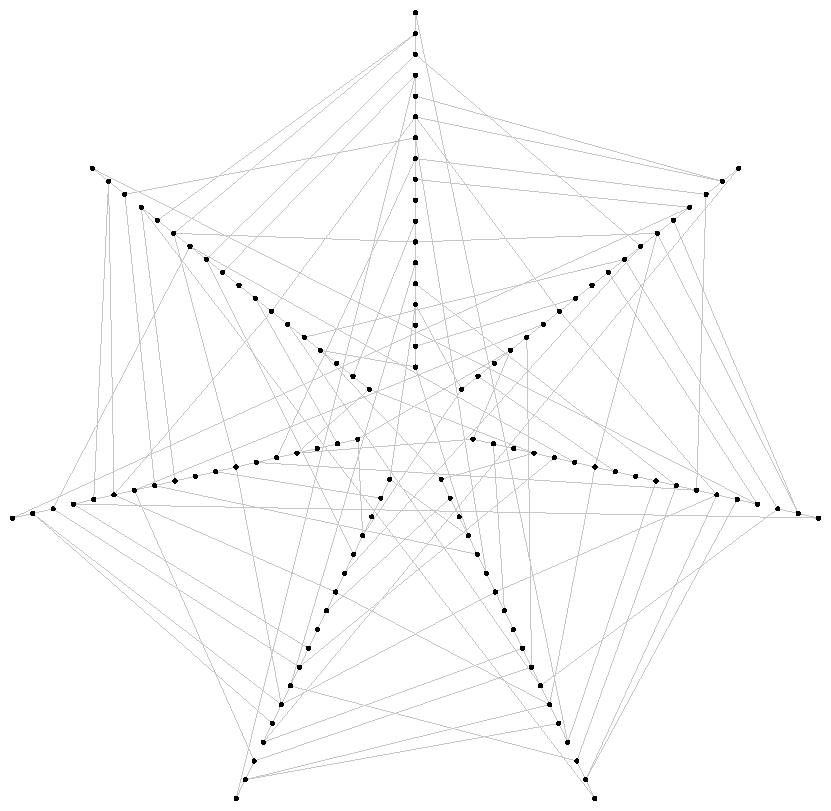
\includegraphics[width=\textwidth]{tutte12cage-clean.pdf}
  \caption{Tutte 12-cage (126v, 3-reg).}
\end{subfigure}
\hfill
\begin{subfigure}[b]{0.32\textwidth}
  \centering
  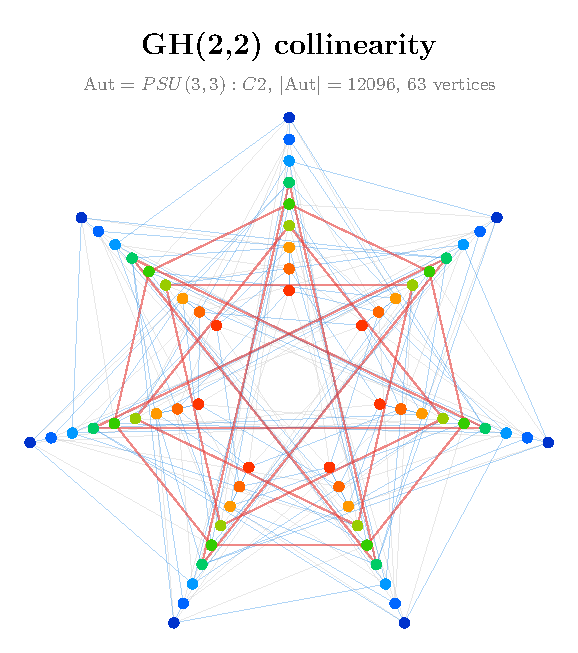
\includegraphics[width=\textwidth]{auto-gh22.pdf}
  \caption{GH(2,2) collinearity (63v, 6-reg).}
\end{subfigure}
\hfill
\begin{subfigure}[b]{0.32\textwidth}
  \centering
  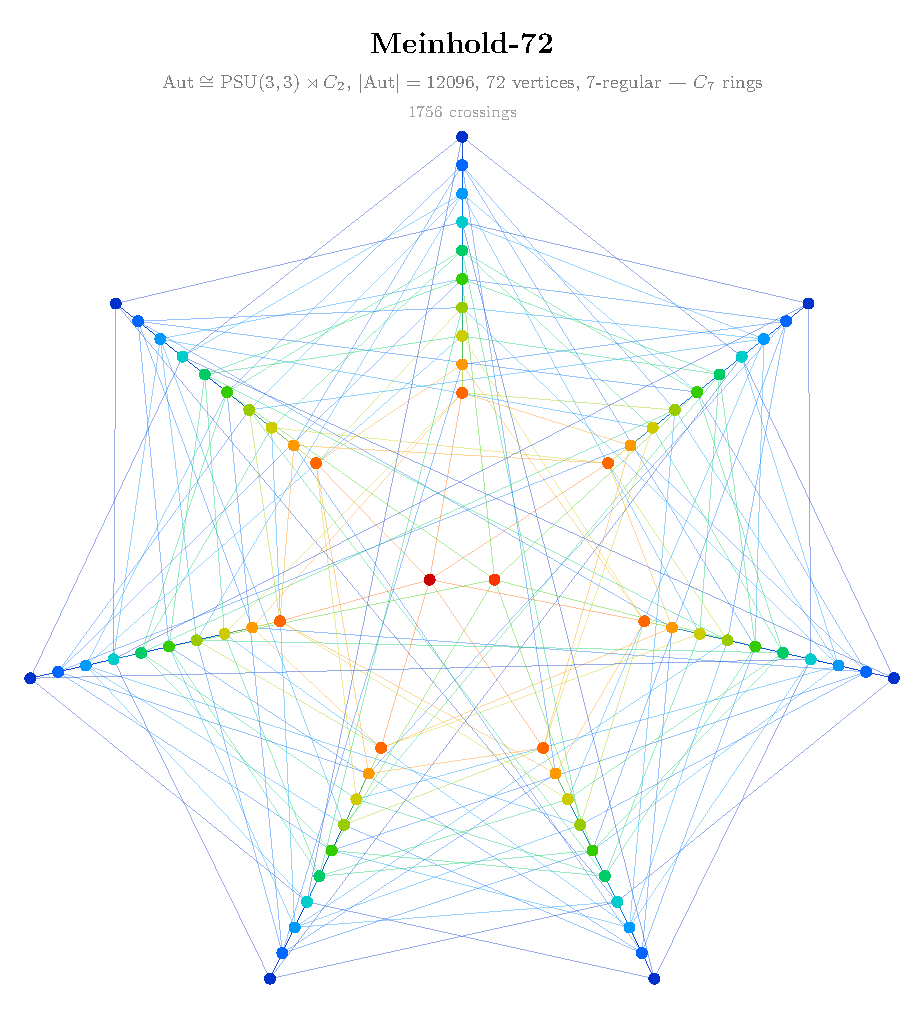
\includegraphics[width=\textwidth]{meinhold72-rings.pdf}
  \caption{Meinhold-72 (72v, 7-reg).}
\end{subfigure}
\caption{The three graphs of $G_2(2)$: the Tutte 12-cage (incidence graph of
  the split Cayley hexagon), the GH(2,2) collinearity graph, and the
  Meinhold-72 semibiplane graph. All three are Ramanujan.}
\label{fig:g2-graphs}
\end{figure}


% ==========================================================================
\section{Spectral analysis}
% ==========================================================================

\subsection{Tutte 12-cage}

\begin{tcolorbox}[colback=black!5, colframe=black!5,
  boxrule=0pt, sharp corners]
\centering
\captionof{table}{Adjacency spectrum of the Tutte 12-cage ($n=126$, $k=3$, girth 12).}
\label{tab:tutte}
\begin{tabular}{@{}rrl@{}}
\toprule
Eigenvalue & Multiplicity & Exact form \\
\midrule
$3$        & $1$  & $k$ (trivial) \\
$\sqrt{6}$ & $21$ & $\approx 2.4495$ \\
$\sqrt{2}$ & $27$ & $\approx 1.4142$ \\
$0$        & $28$ & \\
$-\sqrt{2}$& $27$ & \\
$-\sqrt{6}$& $21$ & \\
$-3$       & $1$  & \\
\bottomrule
\end{tabular}

\begin{proposition}
The Tutte 12-cage is \textbf{Ramanujan}: $\lambda_2 = \sqrt{6} \approx 2.449 < 2\sqrt{2} \approx 2.828$. The spectral gap is $3 - \sqrt{6} \approx 0.551$.
Its spectrum is symmetric about 0 (bipartite: points vs.\ lines), and
the 7 distinct eigenvalues match diameter + 1, confirming distance-regularity.
\end{proposition}
\end{tcolorbox}


\subsection{GH(2,2) collinearity graph}

\begin{tcolorbox}[colback=black!5, colframe=black!5,
  boxrule=0pt, sharp corners]
\centering
\captionof{table}{Adjacency spectrum of the $\GH$ collinearity graph ($n=63$, $k=6$, girth 3).}
\label{tab:gh22}
\begin{tabular}{@{}rrl@{}}
\toprule
Eigenvalue & Multiplicity & Source \\
\midrule
$6$   & $1$  & trivial eigenvalue \\
$3$   & $21$ & \\
$-1$  & $27$ & \\
$-3$  & $14$ & \\
\bottomrule
\end{tabular}

\begin{proposition}
The $\GH$ collinearity graph is \textbf{Ramanujan}: $\lambda_2 = 3 < 2\sqrt{5} \approx 4.472$.
It has exactly 4 distinct eigenvalues (all integers), consistent with diameter~3.
The spectral gap is $6 - 3 = 3$.
\end{proposition}
\end{tcolorbox}

The multiplicity pattern $(1, 21, 27, 14)$ reflects the decomposition of the
permutation character of $G_2(2)$ on 63 points into irreducible representations.


\subsection{Meinhold-72 graph}

\begin{tcolorbox}[colback=black!5, colframe=black!5,
  boxrule=0pt, sharp corners]
\centering
\captionof{table}{Adjacency spectrum of the Meinhold-72 graph ($n=72$, $k=7$, girth 4).}
\label{tab:meinhold}
\begin{tabular}{@{}rrl@{}}
\toprule
Eigenvalue & Multiplicity & Exact form \\
\midrule
$7$           & $1$  & $k$ (trivial) \\
$\sqrt{13}$   & $14$ & $\approx 3.606$ \\
$1$           & $21$ & \\
$-1$          & $21$ & \\
$-\sqrt{13}$  & $14$ & \\
$-7$          & $1$  & \\
\bottomrule
\end{tabular}

\begin{proposition}
The Meinhold-72 graph is \textbf{Ramanujan}: $\lambda_2 = \sqrt{13} \approx 3.606 < 2\sqrt{6} \approx 4.899$. The spectral gap is $7 - \sqrt{13} \approx 3.394$.
Its spectrum is symmetric about 0 (bipartite). While $\lambda_{\min} = -7 = -k$,
the Ramanujan condition concerns nontrivial eigenvalues $|\lambda| < k$, which
are all bounded by $2\sqrt{k-1}$.
\end{proposition}
\end{tcolorbox}


% ==========================================================================
\section{Comparison and discussion}
% ==========================================================================

\begin{tcolorbox}[breakable, colback=yellow!10, colframe=yellow!10,
  boxrule=0pt, sharp corners]
\textbf{Same group, radically different spectra.}
All three graphs have $\Aut(\Gamma) \cong G_2(2)$, yet:
\begin{center}
\small
\begin{tabular}{@{}lrrcccrr@{}}
\toprule
Graph & $n$ & $k$ & $\lambda_2$ & Ram. & Bip. & $g$ & \#ev \\
\midrule
Tutte 12-cage        & 126 & 3 & $\sqrt{6}\approx 2.449$ & Yes & Yes & 12 & 7 \\
GH(2,2) collinearity & 63  & 6 & $3$                     & Yes & No  &  3 & 4 \\
Meinhold-72          & 72  & 7 & $\sqrt{13}\approx 3.606$ & Yes & Yes &  4 & 6 \\
\bottomrule
\end{tabular}
\end{center}
All three are Ramanujan. The collinearity graph is the ``cleanest'' spectrally:
four distinct integer eigenvalues, optimal expansion, with a spectral gap
equal to half the degree. The Tutte cage has the most eigenvalues (7), and
its irrational eigenvalues $\pm\sqrt{6}$ and $\pm\sqrt{2}$ arise from the
distance-regular scheme factoring over $\Q(\sqrt{2}, \sqrt{3})$.

The Meinhold-72 graph sits between: bipartite like the Tutte cage but with
irrational $\pm\sqrt{13}$. The eigenvalue $\sqrt{13}$ and the eigenvalue
$\sqrt{6}$ in the Tutte 12-cage both arise from $G_2(2)$ representation
theory, evaluated on different double cosets.
\end{tcolorbox}

\begin{tcolorbox}[colback=black!5, colframe=black!5,
  boxrule=0pt, sharp corners]
\begin{observation}
The GH(2,2) collinearity graph has spectral gap $6 - 3 = 3$, equal to
half the degree --- an unusually large gap. For comparison, the Petersen
graph (also strongly regular) has gap $3 - 1 = 2 = 2d/3$. This reflects the
exceptional expansion quality of $G_2$-geometries.
\end{observation}
\end{tcolorbox}

\begin{tcolorbox}[colback=blue!5, colframe=blue!5,
  boxrule=0pt, sharp corners]
\textbf{Open direction.}
Can the observed multiplicities $(1, 21, 27, 14)$ of the collinearity graph
be matched to the character table of $G_2(2)$, giving a representation-theoretic
proof of the spectral data?
\end{tcolorbox}


% ======================================================================
%
%  PART V: VOLTAGE GRAPHS AND CUBIC RESIDUES
%
% ======================================================================

\newpage
\part*{Part V: Voltage Graphs and Cubic Residues}
\addcontentsline{toc}{part}{Part V: Voltage Graphs and Cubic Residues}

% ==========================================================================
\section{The voltage graph construction}
% ==========================================================================

\begin{tcolorbox}[colback=green!8, colframe=green!8,
  boxrule=0pt, sharp corners]
\begin{definition}[Voltage graph]
A \emph{voltage graph} $(B, \phi)$ over the group $\Gamma$ consists of
a \emph{base graph} $B$ (possibly with loops and multiple edges) and
a \emph{voltage assignment} $\phi : \vec{E}(B) \to \Gamma$ on the
directed edge set satisfying $\phi(\bar{e}) = \phi(e)^{-1}$.
\end{definition}

\begin{construction}[Derived graph]
\label{con:derived}
Given a voltage graph $(B, \phi)$ over $\Gamma$, the \emph{derived graph}
$B^\phi$ has vertex set $V(B) \times \Gamma$, with edges
$(i, g) \sim (j, g \cdot v)$ for each directed edge $(i \to j, v)$ in $B$.
For $\Gamma = \Z_m$, the derived graph has $m \cdot |V(B)|$ vertices.
\end{construction}
\end{tcolorbox}

\begin{example}[Petersen graph]
The Petersen graph $\GP(5,2)$ is the derived graph of a voltage
graph over $\Z_5$ on two vertices, with a voltage-0 edge between them
and self-loops of voltages 1 and 2.
\end{example}

\begin{figure}[ht]
\centering
\begin{subfigure}[b]{0.32\textwidth}
  \centering
  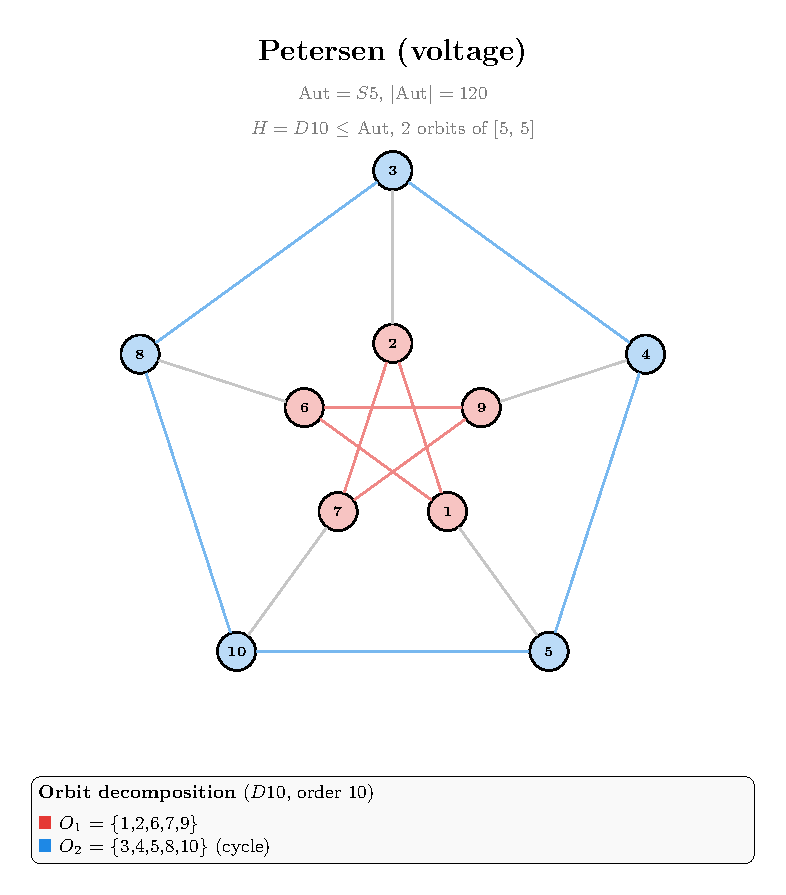
\includegraphics[width=\textwidth]{auto-petersen_voltage.pdf}
  \caption{Petersen graph as $\Z_5$-cover.}
\end{subfigure}
\hfill
\begin{subfigure}[b]{0.32\textwidth}
  \centering
  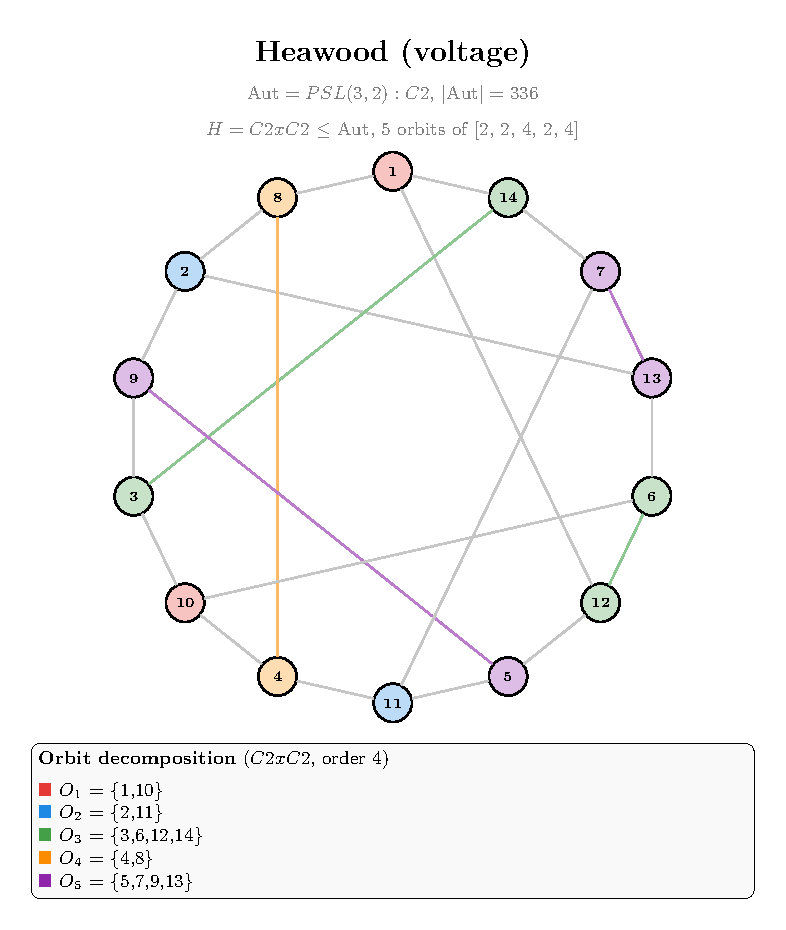
\includegraphics[width=\textwidth]{auto-heawood_voltage.pdf}
  \caption{Heawood graph as $\Z_7$-cover.}
\end{subfigure}
\hfill
\begin{subfigure}[b]{0.32\textwidth}
  \centering
  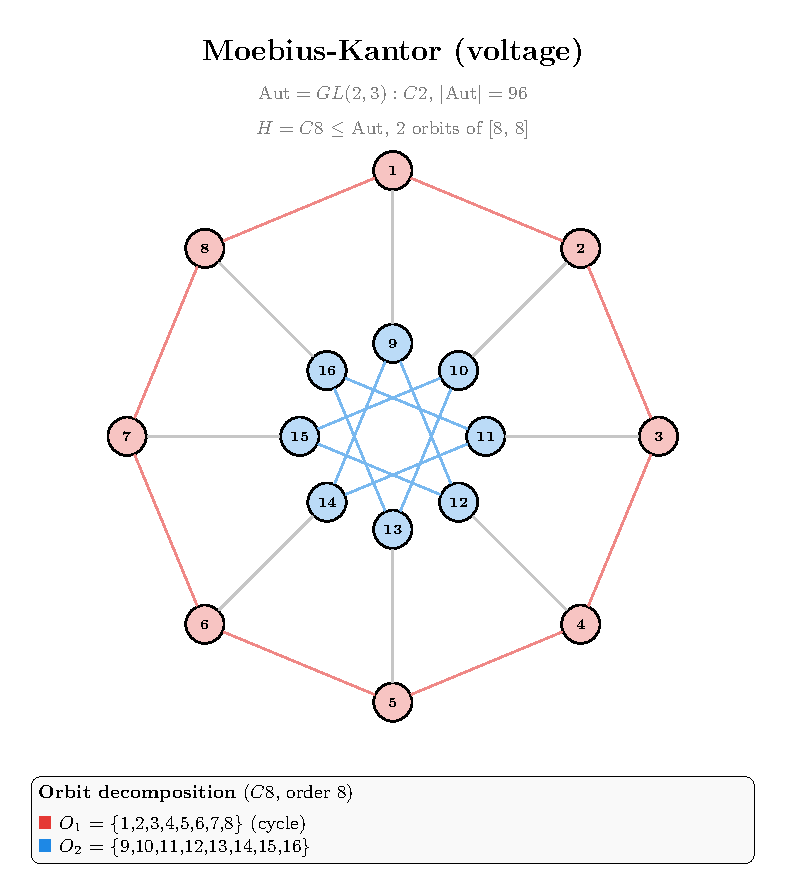
\includegraphics[width=\textwidth]{auto-mk_voltage.pdf}
  \caption{M\"obius--Kantor as $\Z_8$-cover.}
\end{subfigure}

\medskip

\begin{subfigure}[b]{0.45\textwidth}
  \centering
  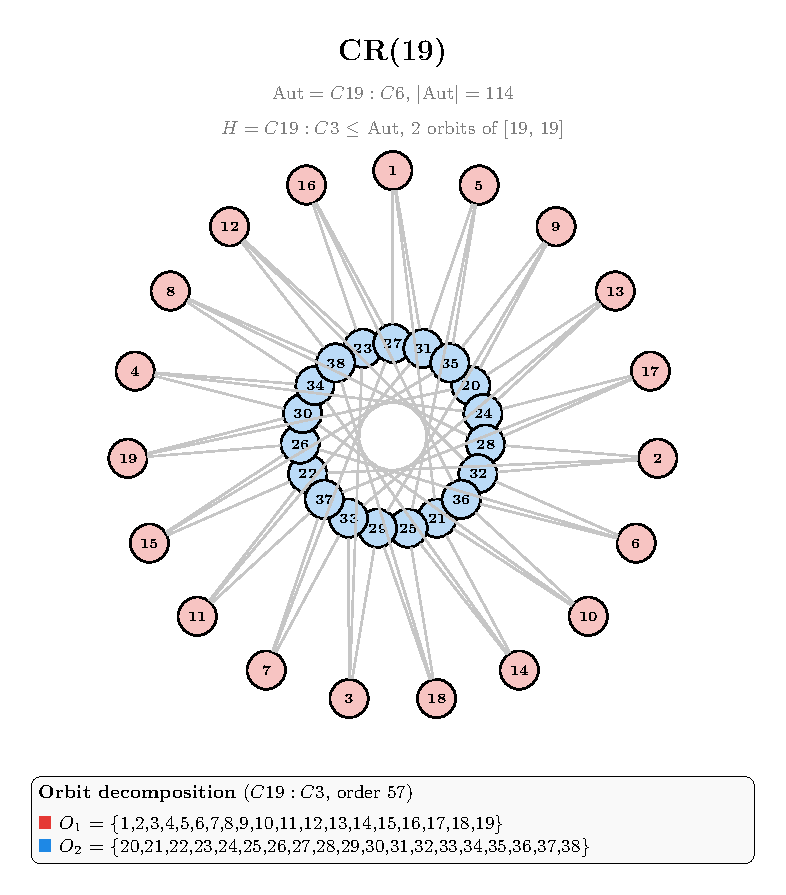
\includegraphics[width=\textwidth]{auto-cr19.pdf}
  \caption{Cubic residue graph CR(19), 19 vertices.}
\end{subfigure}
\hfill
\begin{subfigure}[b]{0.45\textwidth}
  \centering
  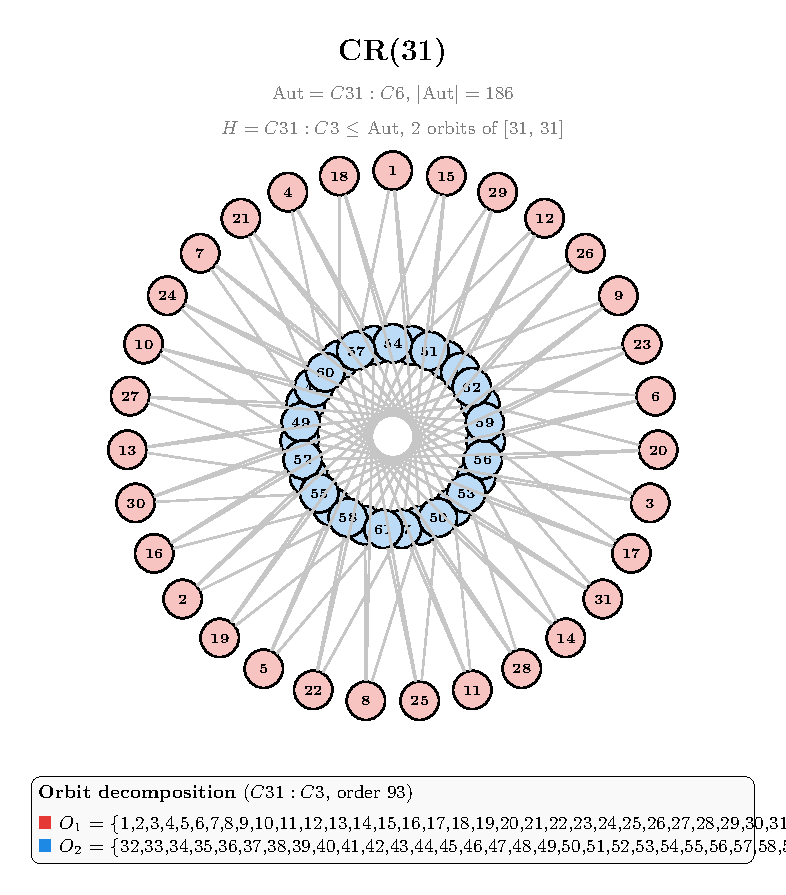
\includegraphics[width=\textwidth]{auto-cr31.pdf}
  \caption{Cubic residue graph CR(31), 31 vertices.}
\end{subfigure}
\caption{Voltage graph derived graphs (top row) and cubic residue graphs
  (bottom row). The cyclic symmetry is manifest in the layout: each graph
  is a $\Z_n$-cover of a small base graph, with the fibre structure visible
  as concentric rings.}
\label{fig:voltage-graphs}
\end{figure}


% ==========================================================================
\section{Spectral theory of cyclic covers}
% ==========================================================================

\begin{tcolorbox}[breakable, colback=black!5, colframe=black!5,
  boxrule=0pt, sharp corners]
\begin{theorem}[Voltage Laplacian spectral theorem]
\label{thm:voltage-spec}
The adjacency eigenvalues of $B^\phi$ consist of the eigenvalues of the
$n \times n$ \emph{voltage Laplacian matrices}
\[
  A_j = \bigl(a_{uv}^{(j)}\bigr)_{u,v \in V(B)}, \qquad
  a_{uv}^{(j)} = \sum_{\substack{e = (u \to v) \\ \text{in } B}} \omega^{j \cdot \phi(e)},
\]
as $j$ ranges over $0, 1, \ldots, m-1$, where $\omega = e^{2\pi i/m}$.
\end{theorem}
\end{tcolorbox}

For the $K_2$ base case with voltage set $V = \{v_1, \ldots, v_k\}$, the
eigenvalues are $\pm |f_j|$ where $f_j = \sum_{v \in V} \omega^{jv}$.
At $j = 0$: $f_0 = k$, giving the trivial eigenvalues $\pm k$.


% ==========================================================================
\section{Cubic residue graphs}
% ==========================================================================

Let $p$ be a prime with $p \equiv 1 \pmod{3}$. The cubic residues form a
subgroup of index~3 in $\F_p^*$, of order $(p-1)/3$.

\begin{tcolorbox}[colback=green!8, colframe=green!8,
  boxrule=0pt, sharp corners]
\begin{definition}
The \emph{cubic residue graph} $\CR(p)$ (voltage lift realisation) is the
$\Z_p$-cover of $K_2$ with voltages $\{1, g, g^2\}$, where $g$ is a
primitive cube root of unity mod~$p$. It is a 3-regular bipartite graph on
$2p$ vertices with girth~6.
\end{definition}
\end{tcolorbox}

The family includes celebrated graphs: $\CR(7)$ is the Heawood graph
(= Foster F14A, Part~II) and $\CR(13)$ is Foster F26A.


% ==========================================================================
\section{Eigenvalues as Gauss sums}
% ==========================================================================

For the $\Z_p$-cover of $K_2$ with voltage set $V = \{1, g, g^2\}$, the
eigenvalues are $\pm |f_j|$ where
$f_j = \omega^j + \omega^{jg} + \omega^{jg^2}$, $\omega = e^{2\pi i/p}$.

\begin{tcolorbox}[colback=black!5, colframe=black!5,
  boxrule=0pt, sharp corners]
\begin{proposition}[Multiplicity structure]
For $j \neq 0$, the orbit of $j$ under multiplication by~$g$ in $\Z_p^*$ has
size exactly~3. Hence each non-trivial eigenvalue $\pm|f_j|$ appears with
multiplicity divisible by~3, and each value of $|f_j|^2$ appears with
multiplicity divisible by~6.
\end{proposition}
\end{tcolorbox}


% ==========================================================================
\section{The Ramanujan property and Weil bounds}
% ==========================================================================

\begin{tcolorbox}[breakable, colback=yellow!10, colframe=yellow!10,
  boxrule=0pt, sharp corners]
\textbf{Why CR(p) is Ramanujan.}
The Ramanujan condition requires $|f_j| \le 2\sqrt{2}$ for all $j \neq 0$.
From the theory of cubic Gauss sums: for the cubic character $\chi$ of
$\F_p^*$, we have $|\tau(\chi)|^2 = p$, and careful analysis shows
$|f_j|^2 \le 8$ for $j \not\equiv 0 \pmod{p}$, i.e.\ $|f_j| \le 2\sqrt{2}$,
which is \emph{exactly} the Ramanujan bound.

Equivalently, $\CR(p)$ is Ramanujan because its eigenvalues are
controlled by cubic character sums bounded by
$2\sqrt{2}$ via the Riemann Hypothesis for curves over finite fields~\cite{Weil}.
\end{tcolorbox}


% ==========================================================================
\section{Spectral data}
% ==========================================================================

\begin{tcolorbox}[breakable, colback=black!5, colframe=black!5,
  boxrule=0pt, sharp corners]
\centering
\captionof{table}{Spectral evolution of $\CR(p)$ as $\Z_p$-covers of $K_2$ (3-regular, $2p$ vertices).
Cross-reference with the master table (Table~\ref{tab:master}).}
\label{tab:cr-lift}
\smallskip
\renewcommand{\arraystretch}{1.2}
\small
\begin{tabular}{@{}r r r r r r r l@{}}
\toprule
$p$ & $|V|$ & Voltages & $\lambda_2$ & $\lambda_{\min}$ & Gap & Girth & Ram. \\
\midrule
 7  & 14  & $\{1,2,4\}$   & $\sqrt{2} \approx 1.414$ & $-3$ & $1.586$ & 6 & \checkmark \\
13  & 26  & $\{1,3,9\}$   & $2.074$ & $-3$ & $0.926$ & 6 & \checkmark \\
19  & 38  & $\{1,7,11\}$  & $2.347$ & $-3$ & $0.653$ & 6 & \checkmark \\
31  & 62  & $\{1,5,25\}$  & $2.591$ & $-3$ & $0.409$ & 6 & \checkmark \\
37  & 74  & $\{1,10,26\}$ & $2.655$ & $-3$ & $0.345$ & 6 & \checkmark \\
43  & 86  & $\{1,6,36\}$  & $2.702$ & $-3$ & $0.298$ & 6 & \checkmark \\
\bottomrule
\end{tabular}
\end{tcolorbox}

\begin{tcolorbox}[colback=black!5, colframe=black!5,
  boxrule=0pt, sharp corners]
\centering
\captionof{table}{Weil bound $|\lambda| \le 2\sqrt{p}$ vs.\ actual non-trivial eigenvalues.}
\label{tab:weil}
\smallskip
\renewcommand{\arraystretch}{1.2}
\small
\begin{tabular}{@{}r r r r l@{}}
\toprule
$p$ & Weil bound $2\sqrt{p}$ & $\max|\lambda_{\text{nontrivial}}|$ & Ramanujan bound $2\sqrt{2}$ & Satisfied? \\
\midrule
 7  & $5.292$ & $1.414$ & $2.828$ & \checkmark \\
13  & $7.211$ & $2.074$ & $2.828$ & \checkmark \\
19  & $8.718$ & $2.347$ & $2.828$ & \checkmark \\
31  & $11.136$ & $2.591$ & $2.828$ & \checkmark \\
37  & $12.166$ & $2.655$ & $2.828$ & \checkmark \\
43  & $13.115$ & $2.702$ & $2.828$ & \checkmark \\
\bottomrule
\end{tabular}
\end{tcolorbox}

\begin{tcolorbox}[colback=yellow!10, colframe=yellow!10,
  boxrule=0pt, sharp corners]
\textbf{Fiedler scaling.}
The Fiedler values $\mu_1 = 3 - \lambda_2$ approach~0 as $p \to \infty$.
The product $p \cdot \mu_1$ stabilises near $4\pi/\sqrt{3} \approx 12.87$,
reflecting equidistribution of cubic residues on the unit circle. Despite
being individually Ramanujan, the $\CR(p)$ family is \emph{not} an expander
family since the spectral gap goes to~0.
\end{tcolorbox}


% ==========================================================================
\section{Connections to classical theory}
% ==========================================================================

The Cayley graph $\CR(p)$ on $\Z_p$ (6-regular, $p$ vertices) is analogous
to the \emph{Paley graph} $\mathrm{Paley}(p)$ for $p \equiv 1 \pmod{4}$,
where the connection set is the set of quadratic residues. The Paley graph
is strongly regular; the cubic analogue is not in general strongly regular
for $p \ge 19$.

The connection to the Foster census is direct: F14A ($p=7$, Heawood) and
F26A ($p=13$) are both $\Z_p$-covers of $K_2$ with cubic residue voltages.
The family continues for each prime $p \equiv 1 \pmod{3}$.


% ======================================================================
%
%  PART VI: HYPERCUBES
%
% ======================================================================

\newpage
\part*{Part VI: Hypercubes}
\addcontentsline{toc}{part}{Part VI: Hypercubes}

\begin{tcolorbox}[colback=yellow!10, colframe=yellow!10,
  boxrule=0pt, sharp corners]
\textbf{Why hypercubes?}
The hypercubes $Q_n$ serve as a contrast to the Lie-type families.
They are Cayley graphs of the abelian group $\Z_2^n$ --- the simplest
possible symmetry group --- yet their spectral theory connects to Boolean
Fourier analysis, coding theory, and association schemes.
The key difference: while Lie-type graphs are \emph{all} Ramanujan,
hypercubes fail at $n = 7$, illustrating the limits of the abelian setting.
\end{tcolorbox}


% ==========================================================================
\section{The hypercube as Cartesian product}
% ==========================================================================

The $n$-dimensional hypercube $Q_n$ has vertex set $\Z_2^n = \{0,1\}^n$,
with adjacency when vertices differ in exactly one coordinate:
$Q_n = K_2^{\square n}$.

\begin{tcolorbox}[colback=black!5, colframe=black!5,
  boxrule=0pt, sharp corners]
\begin{theorem}[Cartesian product spectral theorem]
\label{thm:cart-spec}
If $G$ has eigenvalues $\lambda_1, \ldots, \lambda_m$ and $H$ has
eigenvalues $\mu_1, \ldots, \mu_k$, then $G \mathbin{\square} H$ has
eigenvalues $\{\lambda_i + \mu_j\}$.
\end{theorem}

\begin{corollary}[Spectrum of $Q_n$]
\label{cor:hypercube-spec}
The adjacency eigenvalues of $Q_n$ are
$\lambda_k = n - 2k$ with multiplicity $\binom{n}{k}$, $k = 0, 1, \ldots, n$.
\end{corollary}
\end{tcolorbox}


% ==========================================================================
\section{Boolean Fourier analysis}
% ==========================================================================

Since $Q_n$ is a Cayley graph of the abelian group $\Z_2^n$, its eigenvalues
are given by characters $\chi_S(x) = (-1)^{\sum_{i \in S} x_i}$.
The eigenvalue corresponding to $\chi_S$ is $\lambda_S = n - 2|S|$.

\begin{tcolorbox}[colback=yellow!10, colframe=yellow!10,
  boxrule=0pt, sharp corners]
\textbf{Fourier--Hodge analogy.}
The eigenspaces $W_k = \operatorname{span}\{\chi_S : |S| = k\}$ carry
the $k$-th exterior power of the standard $S_n$-representation:
$W_k \cong \bigwedge^k \R^n$. This is the graph-theoretic analogue of
Hodge theory: the Laplacian eigenspaces decompose $L^2(\Z_2^n)$ into
``$k$-forms.'' The level sets $W_k$ are also the Reed--Muller codes of
order $k$ modulo order $k-1$.
\end{tcolorbox}


% ==========================================================================
\section{The Ramanujan threshold}
% ==========================================================================

\begin{tcolorbox}[colback=black!5, colframe=black!5,
  boxrule=0pt, sharp corners]
\begin{proposition}
The hypercube $Q_n$ is Ramanujan if and only if $n \le 6$.
\end{proposition}
\begin{proof}
The second eigenvalue is $\lambda_2 = n - 2$. The Ramanujan condition
$n - 2 \le 2\sqrt{n-1}$ holds iff $n^2 - 8n + 8 \le 0$, whose roots are
$4 \pm 2\sqrt{2} \approx 1.17$ and $6.83$. So it holds for $n \le 6$.
At $n = 7$: $\lambda_2 = 5 > 2\sqrt{6} \approx 4.899$.
\end{proof}
\end{tcolorbox}

\begin{tcolorbox}[colback=yellow!10, colframe=yellow!10,
  boxrule=0pt, sharp corners]
\textbf{Contrast with Lie-type families.}
That $Q_n$ fails at $n = 7$ does not mean $Q_7$ is a poor expander:
the Cheeger constant $h(Q_n) = 1$ is optimal.
But the second eigenvalue grows \emph{linearly} ($\lambda_2 = n - 2$) while
the Ramanujan bound grows as $O(\sqrt{n})$. This is the fundamental
difference from Lie-type graphs, where character-sum bounds (Weil
conjectures) keep eigenvalues within $2\sqrt{d-1}$.
Abelian groups lack this arithmetic control.
\end{tcolorbox}


% ==========================================================================
\section{Spectral data}
% ==========================================================================

\begin{tcolorbox}[breakable, colback=black!5, colframe=black!5,
  boxrule=0pt, sharp corners]
\centering
\captionof{table}{Adjacency spectrum and key invariants of $Q_n$ for $1 \le n \le 10$.
Cross-reference with the master table (Table~\ref{tab:master}).}
\label{tab:spectra-qn}
\smallskip
\renewcommand{\arraystretch}{1.2}
\small
\begin{tabular}{@{}c r r p{5.6cm} c c c@{}}
\toprule
$Q_n$ & $|V|$ & $\deg$ & Adjacency spectrum ($\lambda^{\text{mult}}$)
  & $\lambda_2$ & Gap & Ram.\ \\
\midrule
$Q_1$ &     2 &  1 & $1^1,\; {-}1^1$
  & $-1$ & 2 & \checkmark \\
$Q_2$ &     4 &  2 & $2^1,\; 0^2,\; {-}2^1$
  & $0$ & 2 & \checkmark \\
$Q_3$ &     8 &  3 & $3^1,\; 1^3,\; {-}1^3,\; {-}3^1$
  & $1$ & 2 & \checkmark \\
$Q_4$ &    16 &  4 & $4^1,\; 2^4,\; 0^6,\; {-}2^4,\; {-}4^1$
  & $2$ & 2 & \checkmark \\
$Q_5$ &    32 &  5 & $5^1,\; 3^5,\; 1^{10},\; {-}1^{10},\; {-}3^5,\; {-}5^1$
  & $3$ & 2 & \checkmark \\
$Q_6$ &    64 &  6 & $6^1,\; 4^6,\; 2^{15},\; 0^{20},\; {-}2^{15},\; {-}4^6,\; {-}6^1$
  & $4$ & 2 & \checkmark \\
$Q_7$ &   128 &  7 & $7^1,\; 5^7,\; 3^{21},\; 1^{35},\; \ldots$ (symmetric)
  & $5$ & 2 & $\times$ \\
$Q_8$ &   256 &  8 & $8^1,\; 6^8,\; 4^{28},\; 2^{56},\; 0^{70},\; \ldots$
  & $6$ & 2 & $\times$ \\
$Q_9$ &   512 &  9 & $9^1,\; 7^9,\; 5^{36},\; 3^{84},\; 1^{126},\; \ldots$
  & $7$ & 2 & $\times$ \\
$Q_{10}$ & 1024 & 10 & $10^1,\; 8^{10},\; 6^{45},\; 4^{120},\; \ldots$
  & $8$ & 2 & $\times$ \\
\bottomrule
\end{tabular}
\end{tcolorbox}

Key patterns: the spectrum is always symmetric about zero (bipartite), the
multiplicities form Pascal's triangle, the spectral gap is constant at~2,
and the Ramanujan property fails precisely at $n = 7$.


% ==========================================================================
\section{The Hamming scheme and expansion}
% ==========================================================================

The hypercube sits inside the Hamming scheme $H(n, 2)$, the association
scheme on $\Z_2^n$ whose eigenmatrix is the matrix of Krawtchouk polynomials.
The adjacency eigenvalue $n - 2k$ equals the Krawtchouk value $K_k(1; n)$.

\begin{tcolorbox}[colback=black!5, colframe=black!5,
  boxrule=0pt, sharp corners]
\begin{proposition}
The algebraic connectivity (Fiedler value) of $Q_n$ is $\mu_1 = 2$ for all
$n \ge 1$. The Fiedler eigenvectors are the coordinate functions
$\chi_{\{i\}}(x) = (-1)^{x_i}$.
\end{proposition}
\end{tcolorbox}

The constant Fiedler value $\mu_1 = 2$ means the bottleneck of a hypercube
is always a single-coordinate bisection, regardless of dimension.
This contrasts sharply with the $\PSL(2,q)$ family where $\mu_1 \sim 4/q$
decays, and with the $\CR(p)$ family where $\mu_1 \sim 12.87/p$ decays.

\begin{tcolorbox}[colback=blue!5, colframe=blue!5,
  boxrule=0pt, sharp corners]
\textbf{Open question.}
The halved cube $\frac{1}{2}Q_n$ (identifying antipodal vertices) is
$\binom{n}{2}$-regular with spectrum governed by even-weight Krawtchouk
polynomials. Can passage to the halved cube restore the Ramanujan property
for $n \ge 7$?
\end{tcolorbox}


% ======================================================================
%
%  BIBLIOGRAPHY
%
% ======================================================================

\begin{thebibliography}{20}

\bibitem{LPS}
A.~Lubotzky, R.~Phillips, P.~Sarnak,
\emph{Ramanujan graphs},
Combinatorica \textbf{8} (1988), 261--277.

\bibitem{Deligne}
P.~Deligne,
\emph{La conjecture de Weil. I},
Publ.\ Math.\ IH\'ES \textbf{43} (1974), 273--307.

\bibitem{Sabidussi}
G.~Sabidussi,
\emph{On a class of fixed-point-free graphs},
Proc.\ Amer.\ Math.\ Soc.\ \textbf{9} (1958), 800--804.

\bibitem{BiggsSm}
N.~Biggs, D.~H.~Smith,
\emph{On trivalent graphs},
Bull.\ London Math.\ Soc.\ \textbf{3} (1971), 155--158.

\bibitem{BCN}
A.~E.~Brouwer, A.~M.~Cohen, A.~Neumaier,
\emph{Distance-Regular Graphs},
Springer, 1989.

\bibitem{BH}
A.~E.~Brouwer, W.~H.~Haemers,
\emph{Spectra of Graphs},
Springer, 2012.

\bibitem{Lafforgue}
L.~Lafforgue,
\emph{Chtoucas de Drinfeld et correspondance de Langlands},
Invent.\ Math.\ \textbf{147} (2002), 1--241.

\bibitem{Alon}
N.~Alon,
\emph{Eigenvalues and expanders},
Combinatorica \textbf{6} (1986), 83--96.

\bibitem{Weil}
A.~Weil,
\emph{On some exponential sums},
Proc.\ Nat.\ Acad.\ Sci.\ USA \textbf{34} (1948), 204--207.

\bibitem{Biggs}
N.~Biggs,
\emph{Algebraic Graph Theory} (2nd edition),
Cambridge University Press, 1993.

\bibitem{foster1988}
R.~M.~Foster,
Census of trivalent symmetrical graphs,
in \emph{Graphs and Combinatorics}, Lecture Notes in Math.\ \textbf{406},
Springer, 1988, pp.~871--898.

\bibitem{conder2002}
M.~Conder, P.~Dobcs\'{a}nyi,
Trivalent symmetric graphs on up to 768 vertices,
\emph{J.\ Combin.\ Math.\ Combin.\ Comput.}\ \textbf{40} (2002), 41--63.

\bibitem{GRAPE}
L.~Soicher,
GRAPE: A system for computing with graphs and groups,
in \emph{Groups and Computation}, DIMACS Ser., AMS, 1993, pp.~287--291.

\end{thebibliography}

\end{document}
